\documentclass[oneside, 11pt]{book}
\usepackage[a4paper, top=3cm, bottom=3cm, inner=2cm, outer=2cm, head=15pt]{geometry}

\usepackage{packages}

\addbibresource{references.bib}

\renewcommand{\maketitle}{\begin{titlepage}
	\begin{center}
		\vspace*{1cm}
		
		
\includegraphics[width=0.7\textwidth]{uob-logo.eps}
		
		\vspace{1.5cm}
		
		\huge
		Can distributed systems be used to increase data processing performance for larger than memory datasets?
		
		%\vspace{0.5cm}
		
		%\large
		%An investigation into the development of a tool for processing queries across a cluster of nodes.
		
		\vspace{2cm}
		
		\large
		\textbf{Oliver Little}
		
		\vspace{0.25cm}
		
		\small 2011802
		
		\vspace{0.25cm}
		
		\large
		D.A. B.Sc Computer Science with Digital Technology Partnership (PwC)
		
		\vspace{2cm}
		
		Supervisor: Vincent Rahli
		
		\vspace{2cm}
		
		\large
		School of Computer Science
		
		\large
		College of Engineering and Physical Sciences
		
		\large
		April 2023
	\end{center}
\end{titlepage}}
\setlength\evensidemargin{\oddsidemargin}

\pagestyle{plain}

% Figure numbering
\usepackage{chngcntr}
\counterwithin{figure}{section}

% Listings config
% From: https://tex.stackexchange.com/questions/83882/how-to-highlight-python-syntax-in-latex-listings-lstinputlistings-command

% Default fixed font does not support bold face
\DeclareFixedFont{\ttb}{T1}{txtt}{bx}{n}{12} % for bold
\DeclareFixedFont{\ttm}{T1}{txtt}{m}{n}{12}  % for normal

% Custom colors
\usepackage{color}
\definecolor{deepred}{rgb}{0.6,0,0}
\definecolor{deepgreen}{rgb}{0,0.5,0}

% Python style for highlighting
\newcommand\pythonstyle{\lstset{
		language=Python,
		basicstyle=\small\ttm,
		breakatwhitespace=true,
		breaklines=true,
		morekeywords={self, cassandra_table, evaluate, Pow, Concat, ToDouble, Substring, ToString, select, filter, group_by, as_name, datetime},              % Add keywords here
		keywordstyle=\color{blue},
		emph={ClusterManager, Max, Avg, Min, Sum, Count, DistinctCount, StringConcat, DistinctStringConcat, F, V, Function, date, __init__},          % Custom highlighting
		emphstyle=\color{deepred},    % Custom highlighting style
		stringstyle=\color{deepgreen},
		frame=tb,                         % Any extra options here
		showstringspaces=false
}}

% Python environment
\lstnewenvironment{python}[1][]
{
	\pythonstyle
	\lstset{#1}
}
{}

% Python for inline
\newcommand\pythoninline[1]{{\pythonstyle\lstinline!#1!}}

% SQL
% From: https://gist.github.com/vivngo/e37e1c7b79bf7e8b910c6566c59c46be
\definecolor{dkgreen}{rgb}{0,0.6,0}
\definecolor{gray}{rgb}{0.5,0.5,0.5}
\newcommand\sqlstyle{\lstset{language=SQL,
	basicstyle={\small\ttm},
	belowskip=3mm,
	breakatwhitespace=true,
	breaklines=true,
	classoffset=0,
	columns=flexible,
	commentstyle=\color{dkgreen},
	frame=tb,                        
	keywordstyle=\color{blue},
	numbers=none, %If you want line numbers, set `numbers=left`
	numberstyle=\tiny\color{gray},
	showstringspaces=false,
	stringstyle=\color{deepgreen},
	tabsize=3
}}

% SQL environment
\lstnewenvironment{SQL}[1][]
{
	\sqlstyle
	\lstset{#1}
}
{}




\begin{document}
	\maketitle
	
	{\let\cleardoublepage\relax \frontmatter}
	
	\begingroup
	\let\cleardoublepage\clearpage
	\tableofcontents
	\endgroup
	\begingroup
	\let\cleardoublepage\clearpage
	\listoffigures
	\endgroup
	
	\chapter*{Abstract}
%The abstract should, in 200-300 words, explain to the reader what 'problem' you have identified, the approach you took to solving this problem and what it produced, and evaluation of your efforts and some kind of conclusion about what all this means. Normally you're going to be limited to a few sentences on each. You don't need to convey everything in the abstract; focus on the high-level things. The abstract is almost a self-contained document of its own; it should be interpretable without the rest of the report.

% High level of data processing from introduction
The explosion in data volumes in the past 15 years has resulted in increasing demands for solutions to process and analyse this data. Existing single-system solutions like SQL struggle to cope with extremely large volumes of data, suffering from performance slowdowns and long execution times. 

While there is an upper limit to the performance of a single system, distributed systems do not face the same issues and can scale to as many nodes as required, therefore presenting an excellent alternative solution to this problem.

This report presents a distributed systems solution for performing various types of data processing tasks, designed around splitting the source data into manageable partitions which can be computed by any node in the cluster. By focusing on closely integrating the persistent storage and computation nodes, the solution is able to assign partitions of the source data to the closest node, thereby reducing the effect of network latency. 

As part of the solution, a domain specific language (DSL) is also developed, enabling users to succinctly describe complex data manipulations, including Select, Filter and Group By operations.

% Testing
The solution is evaluated in a number of ways. Firstly, raw performance testing is conducted against SQL server, a typical single-system approach, identifying that further optimisations are required for the solution to truly compete with existing options. Testing is also performed surrounding the optimal level of parallelisation, showing that this depends on the application and data volumes. Finally, the solution has the potential to automatically adjust the number of nodes in the cluster based on demand to provide cost benefits in a public cloud environment; the results of this testing show that at small data volumes there is minimal performance impact when the number of nodes are reduced.


		
	\mainmatter
		
	\chapter{Introduction}

% Very high level overview of project aims

\section{Background}

% Why is this area important, why am I investigating it
% More general big data references here - difficulties faced due to larger than memory data sets
% References to ETL if possible, and how this is an increasingly important workflow.

\section{Prior Work}
% Literature review
% General topics within distributed data processing

Distributed Data Processing has existed conceptually since as early as the 1970s. A key paper by Philip Enslow Jr. from this period \cite{enslow1978distributed} sets out characteristics across three 'dimensions' of decentralisation - hardware, control and database. Enslow argued that these dimensions defined a distributed system, while also acknowledging that the technology of the period was not equipped to fulfil the goals he laid out.

Research into solutions for distributed data processing has generally resulted in two kinds of solutions \cite{yaqoob2016big}:
\begin{itemize}
	\item \textbf{Batch processing:} where data is gathered, processed and output all at the same time. This includes solutions like MapReduce \cite{dean2008mapreduce} and Spark \cite{zaharia2016spark}. Batch processing works best for data that can be considered 'complete' at some stage.
	\item \textbf{Stream processing:} where data is processed and output as it arrives. This includes solutions like Apache Flink \cite{carbone2015flink}, Storm \cite{toshniwal2014storm}, and Spark Streaming \cite{armbrust2018sparkstreaming}. Stream processing works best for data that is being constantly generated, and needs to be analysed as it arrives.
\end{itemize}

MapReduce \cite{dean2008mapreduce}, a framework introduced by Google  in the mid 2000s, could be considered the breakthrough framework for performing massively scalable, parallelised data processing. This framework later became one of the core modules for the Apache Hadoop suite of tools. It provided a simple API, where developers could describe a job as a \textit{map} and a \textit{reduce} step, and the framework would handle the specifics of managing the distributed system. 

While MapReduce was Google's offering, other large technology companies had similar solutions, including Microsoft, who created DryadLINQ in 2009 \cite{fetterly2009dryadlinq}. However, due to the massive success of MapReduce, Microsoft discontinued DryadLINQ in 2011.

MapReduce was not without flaws, and many papers were published in the years following its initial release which performed performance benchmarks, and analysed its strengths and weaknesses \cite{lee2012parallel}. Crucially, MapReduce appears to particularly struggle with iterative algorithms, like the PageRank algorithm used by Google's own search engine. A number of popular extensions to MapReduce were introduced to improve the performance on iterative algorithms, like Twister \cite{ekanayake2010twister} and HaLoop \cite{bu2010haloop} both in 2010. 

MapReduce's popularity also resulted in a number of tools being created to improve its usability and accessibility. Hive \cite{thusoo2010hive} is one such tool, which features a SQL-like language called HiveQL to allow users to write declarative programs that compiled into MapReduce jobs. Pig Latin \cite{olston2008pig} is similar, and features a mixed declarative and imperative language style that again compiles down into MapReduce jobs. 

Further tools in the wider areas of the field were introduced around 2010, including another project by Google named Pregel \cite{malewicz2010pregel}, specialised for performing distributed data processing on large-scale graphs.

% Spark - initial creation, talk specifically about RDDs
In 2010, the first paper on Spark \cite{zaharia2010spark} was released. Spark aims to improve upon MapReduce's weaknesses, by storing data in memory, and providing fault tolerance by tracking the 'lineage' of data. This means for any set of data, Spark knows how the data was constructed from another persistent, fault tolerant data source, and can use that to reconstruct any lost data in the event of failure. This in-memory storage, known as a resilient distributed dataset (RDD) \cite{zaharia2012rdd} allows Spark to improve on MapReduce's performance for iterative jobs, whilst also allowing it to quickly perform ad-hoc queries.  Effectively, Spark is strong at performing long batch jobs, as well as short interactive queries. This is something that I would like my solution to feature, as users of the framework will need to design long-running scripts to run on large amounts of data, as well as run ad-hoc queries to perform investigation.

% Spark - extensions - SQL, Streaming
Spark quickly grew in popularity, with a number of extensions being added to improve its usability, including a SQL-style engine with a query optimiser \cite{armbrust2015sparksql}, as well as an engine to modify Spark to support stream processing \cite{armbrust2018sparkstreaming}. A second paper released in 2016 \cite{zaharia2016spark} stated that Spark was in use in thousands of organisations, with the largest deployment running an 8,000 node cluster holding 100PB of data. 
% TODO: reference this claim
One area where Spark struggles is with grouped data, as performing grouped operations requires shuffling the data between all nodes. I aim to improve upon this in my solution through the design of the system as a whole.

% Stream processing tools - not entirely what I'm looking at, but still within the field - Kafka, Storm
More recent research indicates that the future of the field is moving away from batch processing, and towards stream processing for data that is constantly being generated. A 2015 paper by Google \cite{akidau2015dataflow} argues that the volumes of data, the fact that datasets can no longer ever be considered 'complete', along with demands for improved insight into the data means that streaming 'dataflow' models are the way forward. Google publicly stated in their 2014 'Google I/O' Keynote \cite{googleio2014} that they were phasing out MapReduce in their internal systems. The data I will be using is not being received at this constant rate, and as such designing for a streaming solution is not required in this case.

\section{Project Aims}

% Reiterate high level aim, explain how my solution will differ from prior work discussed
% Focus on grouped data, and improving access efficiency for that
% Easy-to-use Python interface

	
	\chapter{Design}

After conducting my review of previous work, I spent time producing a high-level design for my solution. In particular, I analysed what features it needed to have, what technologies I would use, and the overall architecture. The aim of this was to ensure that the limited development time I had was always spent producing the most useful features.

\section{MoSCoW Requirements}

Before considering specific technologies and frameworks, I produced a list of MoSCoW requirements. Each requirement in the table below has two extra columns. The first column represents whether the requirement is Functional (F) or Non-Functional (NF), and the second column represents requirements that Must (M), Should (S) or Could (C) be completed.

\begin{center}
	\begin{xltabular}{0.82\paperwidth}{ | p{1.5cm} | p{1.5cm} | X | } 
		\hline
		F / NF& Priority & Requirement Description \\ \hline
		
 		\multicolumn{3}{|c|}{Domain Specific Language - Expressions} \\ \hline
		F & M & The language must support 5 data types: integers, floats, booleans, strings and date-time objects. \\ \hline
		F & M & The language must allow users to reference a field in the current dataset. \\ \hline
		F & M & The language must allow users to reference a constant value, which can take one of the data types defined above. \\ \hline
		F & M & The language must support arithmetic operations like add, subtract, multiply, division and modulo. \\ \hline
		F & M & The language must support string slicing and concatenation. \\ \hline
		F & S & The language should utilise polymorphism in add operations to apply string concatenation, or arithmetic addition depending on the data types of the arguments. \\ \hline
		F & C & The language could be designed in such a way to allow the user to define their own functions. \\ \hline
		NF & S & The language should be intuitive to use, with SQL-like syntax. \\ \hline
		
		\multicolumn{3}{|c|}{Domain Specific Language - Comparisons} \\ \hline
		F & M & The user must be able to provide expressions as inputs to comparison operators. \\ \hline
		F & M & The language must support equals, and not equals comparisons \\ \hline
		F & M & The language must support inequalities, using numerical ordering for number types, and lexicographic ordering for strings. \\ \hline
		F & M & The language must support null and not null checks. \\ \hline
		F & S & The language should support string comparisons, including case sensitive and insensitive versions of contains, starts with, and ends with. \\ \hline
		F & S & The language should allow the user to combine multiple comparison criteria using $AND$ and $OR$ operators. \\ \hline
		
		\multicolumn{3}{|c|}{Data Processing} \\ \hline
		F & M & The system must allow the user to write queries in Python. \\ \hline
		F & M & The system must allow users to apply Select operations on datasets, applying custom expressions to the input data. \\ \hline
		F & M & The system must allow users to apply Filter operations on datasets, applying custom comparisons to the input data. \\ \hline
		F & M & The system must allow users to apply Group By operations on datasets, which take a number of expressions as unique keys, and a number of aggregate. \\ \hline
		F & M & The Group By operation must allow users to apply Minimum, Maximum, Sum and Count aggregate functions to Group By operations. \\ \hline
		F & C & The system could allow users to apply Distinct Count, String Aggregate, and Distinct String Aggregate aggregate functions to Group By operations. \\ \hline
		F & S & The system should allow users to join two datasets together according to custom criteria. \\ \hline
		NF & S & The complexities of the system should be hidden from the user; from their perspective the operation should be identical whether the user is running the code locally or over a cluster. \\ \hline
		
		\multicolumn{3}{|c|}{Cluster} \\ \hline
		F & M & The system must allow the user to upload source data to a permanent data store. \\ \hline
		F & M & The orchestrator node must split up the full query and delegate partial work to the worker nodes. \\ \hline
		F & M & The orchestrator node must collect partial results from the cluster nodes to produce the overall result for the user. \\ \hline
		F & M & The orchestrator node must handle worker node failures and other computation errors by reporting them to the user. \\ \hline
		F & S & The orchestrator should perform load balancing to ensure work is evenly distributed among all nodes. \\ \hline
		F & C & The orchestrator could handle worker node failures by redistributing work to active workers. \\ \hline
		F & M & The worker nodes must accept partial work, compute and return results to the orchestrator. \\ \hline
		F & M & The worker nodes must pull source data from the permanent data store. \\ \hline
		F & M & The worker nodes must report any computation errors to the orchestrator. \\ \hline
		F & S & The worker nodes should cache results for reuse in later queries. \\ \hline
		F & S & The worker nodes should spill data to disk storage when available memory is low. \\ \hline
	\end{xltabular}
\end{center}

\section{Design Choices}

From the MoSCoW requirements I had a number of decisions to make regarding what languages and technologies I would use to implement my solution.

\subsection{Language}

\paragraph{Frontend} 
Python was selected as the language of choice for the frontend. This is because the intended users of my solution are most experienced with Python and SQL, which should make it easier for them to adopt and use my solution.

\paragraph{Orchestrator and Worker Nodes}
Both the orchestrator and worker nodes would use the same language, which would reduce overhead as the same codebase could be used for both parts of the system. When selecting a language, I firstly had to decide whether I would use a language with automatic or manual garbage collection (GC). Choosing a manual GC language would theoretically allow for increased performance, but I also felt that it would slow my development down significantly, as I would have to spend time handling GC myself. Therefore, I ruled out these languages.

The remaining options were a range of object-oriented and functional languages. I knew that much of the implementation would require iterating over lists of items, and functional languages are strong at this because of their use of operations like $map$ and $reduce$. However, I did not have any experience using purely functional languages like Haskell for large software engineering projects, and so ruled these out. I also knew that the solution would need to perform large amounts of CPU intensive processing, so a language with strong support for parallelisation was preferable. This ruled out languages like Python and JavaScript which are largely single-threaded; both support some form of parallelisation, but much more manual intervention by the developer is required.

In the end, I chose Scala, which is built on top of Java. It features a mix of both object-oriented, and functional paradigms, with built-in support for parallelisation and threading. This would allow me to leverage my previous experience writing large solutions in object-oriented languages, while making use of the functional programming style when convenient. Furthermore, packages originally written for Java can run in Scala, and I felt this wider compatibility would be useful with my later design choices.
 
\subsection{Runtime}
\paragraph{Containerisation}
With the nature of my project being to produce a distributed system, the clear choice for how to run my code was within containers. Docker is by far the most popular option for creating images to run as containers, but is not suitable for running and managing large numbers of containers. For this, I would need a container orchestration tool, and there are two main options: Docker Swarm, and Kubernetes. Docker Swarm is more closely integrated within the Docker ecosystem, but Kubernetes is more widely used in industry. I felt that the experience I would gain learning to use Kubernetes would be more useful, and therefore chose it as my container orchestration tool.

\paragraph{Network Communication} 
I also had to select a method of communicating between the Python frontend, the orchestrator and the worker nodes. At first, I considered various REST API frameworks, but upon further research, found that a remote procedure call (RPC) framework would be more suited to my needs. This is because REST is resource-centric, providing a standard set of operations - create, read, update, delete (CRUD). My system is less resource-centric, and more focused on operations, so the CRUD model wouldn't fit the requirements correctly. In contrast, RPC frameworks are designed to allow function calls over a remote network, while hiding the complexity of the remote operation from the developer. My research into these frameworks found that they are usually not designed around a particular data model like REST, which would allow me to implement my own function calls. 

In the end, I chose gRPC, designed and maintained by Google, as the RPC framework for my solution. I did this for a number of reasons. Firstly, there are well-maintained implementations for both Python and Scala, which would make using it in all parts of my system straightforward. Secondly, it uses protocol buffers as its message system, which is a serialisation format also maintained by Google. Protocol buffers are designed to be extremely storage efficient, which would reduce network overhead compared to a solution that used something like XML or JSON. As protocol buffers are also a serialisation format, gRPC provides APIs to store messages on disk, which I felt might be a useful feature.


\subsection{Persistent Storage}
I had a wide range of options for implementing persistent data storage. The first key decision in this area was whether to design this myself, or use an existing storage solution. A custom solution would come with the benefit of being more closely integrated with the rest of the system, but at the cost of increased development time. I chose not to implement my own solution, as I felt that I was already limited on time, and designing a resilient persistent storage module is a large challenge in its own right.

There are a wide range of options that exist for persistent data storage. I considered a number of types of file systems and databases which I eventually elected not to use:
\begin{itemize}
	\item Single System SQL Databases \textit{(Microsoft SQL Server, PostgreSQL, MySQL)}: while this option would be fastest to start using due to my prior knowledge, and extensive support, the database would quickly become a bottleneck in my system, as the rate at which data can be read from the server would determine how quickly computations could be performed.
	\item Distributed File Systems \textit{(Hadoop Distributed File System)}: these provide a mechanism for storing files resiliently across a number of machines, which would reduce the bottleneck when reading data. However, they provide no straightforward way of querying the stored data, meaning I would have to implement this myself.
	\item Distributed NoSQL Databases \textit{(MongoDB, CouchDB)}: these are distributed, meaning the load of reading the data could be spread across a number of machines. However, the data I will be processing is strictly tabular in format, meaning I don't need the features of a NoSQL architecture (document formats), and it is likely to result in added complexity when retrieving data from the database.
\end{itemize}

\paragraph{Apache Cassandra} 
In the end, I selected Apache Cassandra %reference
as my persistent storage module. This has a number of benefits for the solution I am designing. Firstly, the data model is very similar to single-system SQL databases, and as such closely matches the data model I intend to use. Furthermore, it is a distributed database, so source data will be stored across a number of machines (nodes). This will allow me to spread the load when retrieving data from the database, reducing the impact of read speed. 

Aside from these benefits, the main reason I selected Cassandra as my persistent data store was because of how it handles partitioning data. Each node in the database is assigned a token range, which determines what records it holds. When data is inserted into the database, Cassandra hashes the primary key of each record, producing a 64-bit token that maps it to a node. A diagram showing this process is included below:

% diagram

Cassandra allows these tokens to be filtered in ranges as part of queries, so this will allow me to split up the data that each of the worker nodes pull in .

Cassandra can be run on Kubernetes using K8ssandra \cite{k8ssandra}. This is a tool which can be used to initialise, configure and manage Cassandra clusters. This is particularly useful because the Cassandra cluster can be configured to run on the same machines as the worker nodes. This enables the source data to be co-located with the workers that will actually perform the computation, reducing network latency when transferring the source data.

In terms of interfacing with the rest of the system, there are drivers for both Python %reference
and Java %reference.
which are maintained by one of the largest contributors to Apache Cassandra. The Java driver has a core module which provides basic functionality for making queries and receiving results from the database. There are submodules with more complex functionality including query builders, but I chose not to use these as I was unlikely to actually use the features, and did not want to handle the extra complexity these submodules would introduce.

There are also some Scala specific frameworks for executing Cassandra queries, including Phantom %reference
and Quill. %reference
Again, I chose not to use these as I felt the extra functionality was not required, and they may introduce extra complexity which could be difficult to debug.


\section{Architecture}


	
	\chapter{Implementation}

A number of components were created to implement the proposed architecture. This chapter will provide a high level overview of the system, then examine each component in further detail.

\section{Overall Solution}
\begin{figure}[h]
	\centering
	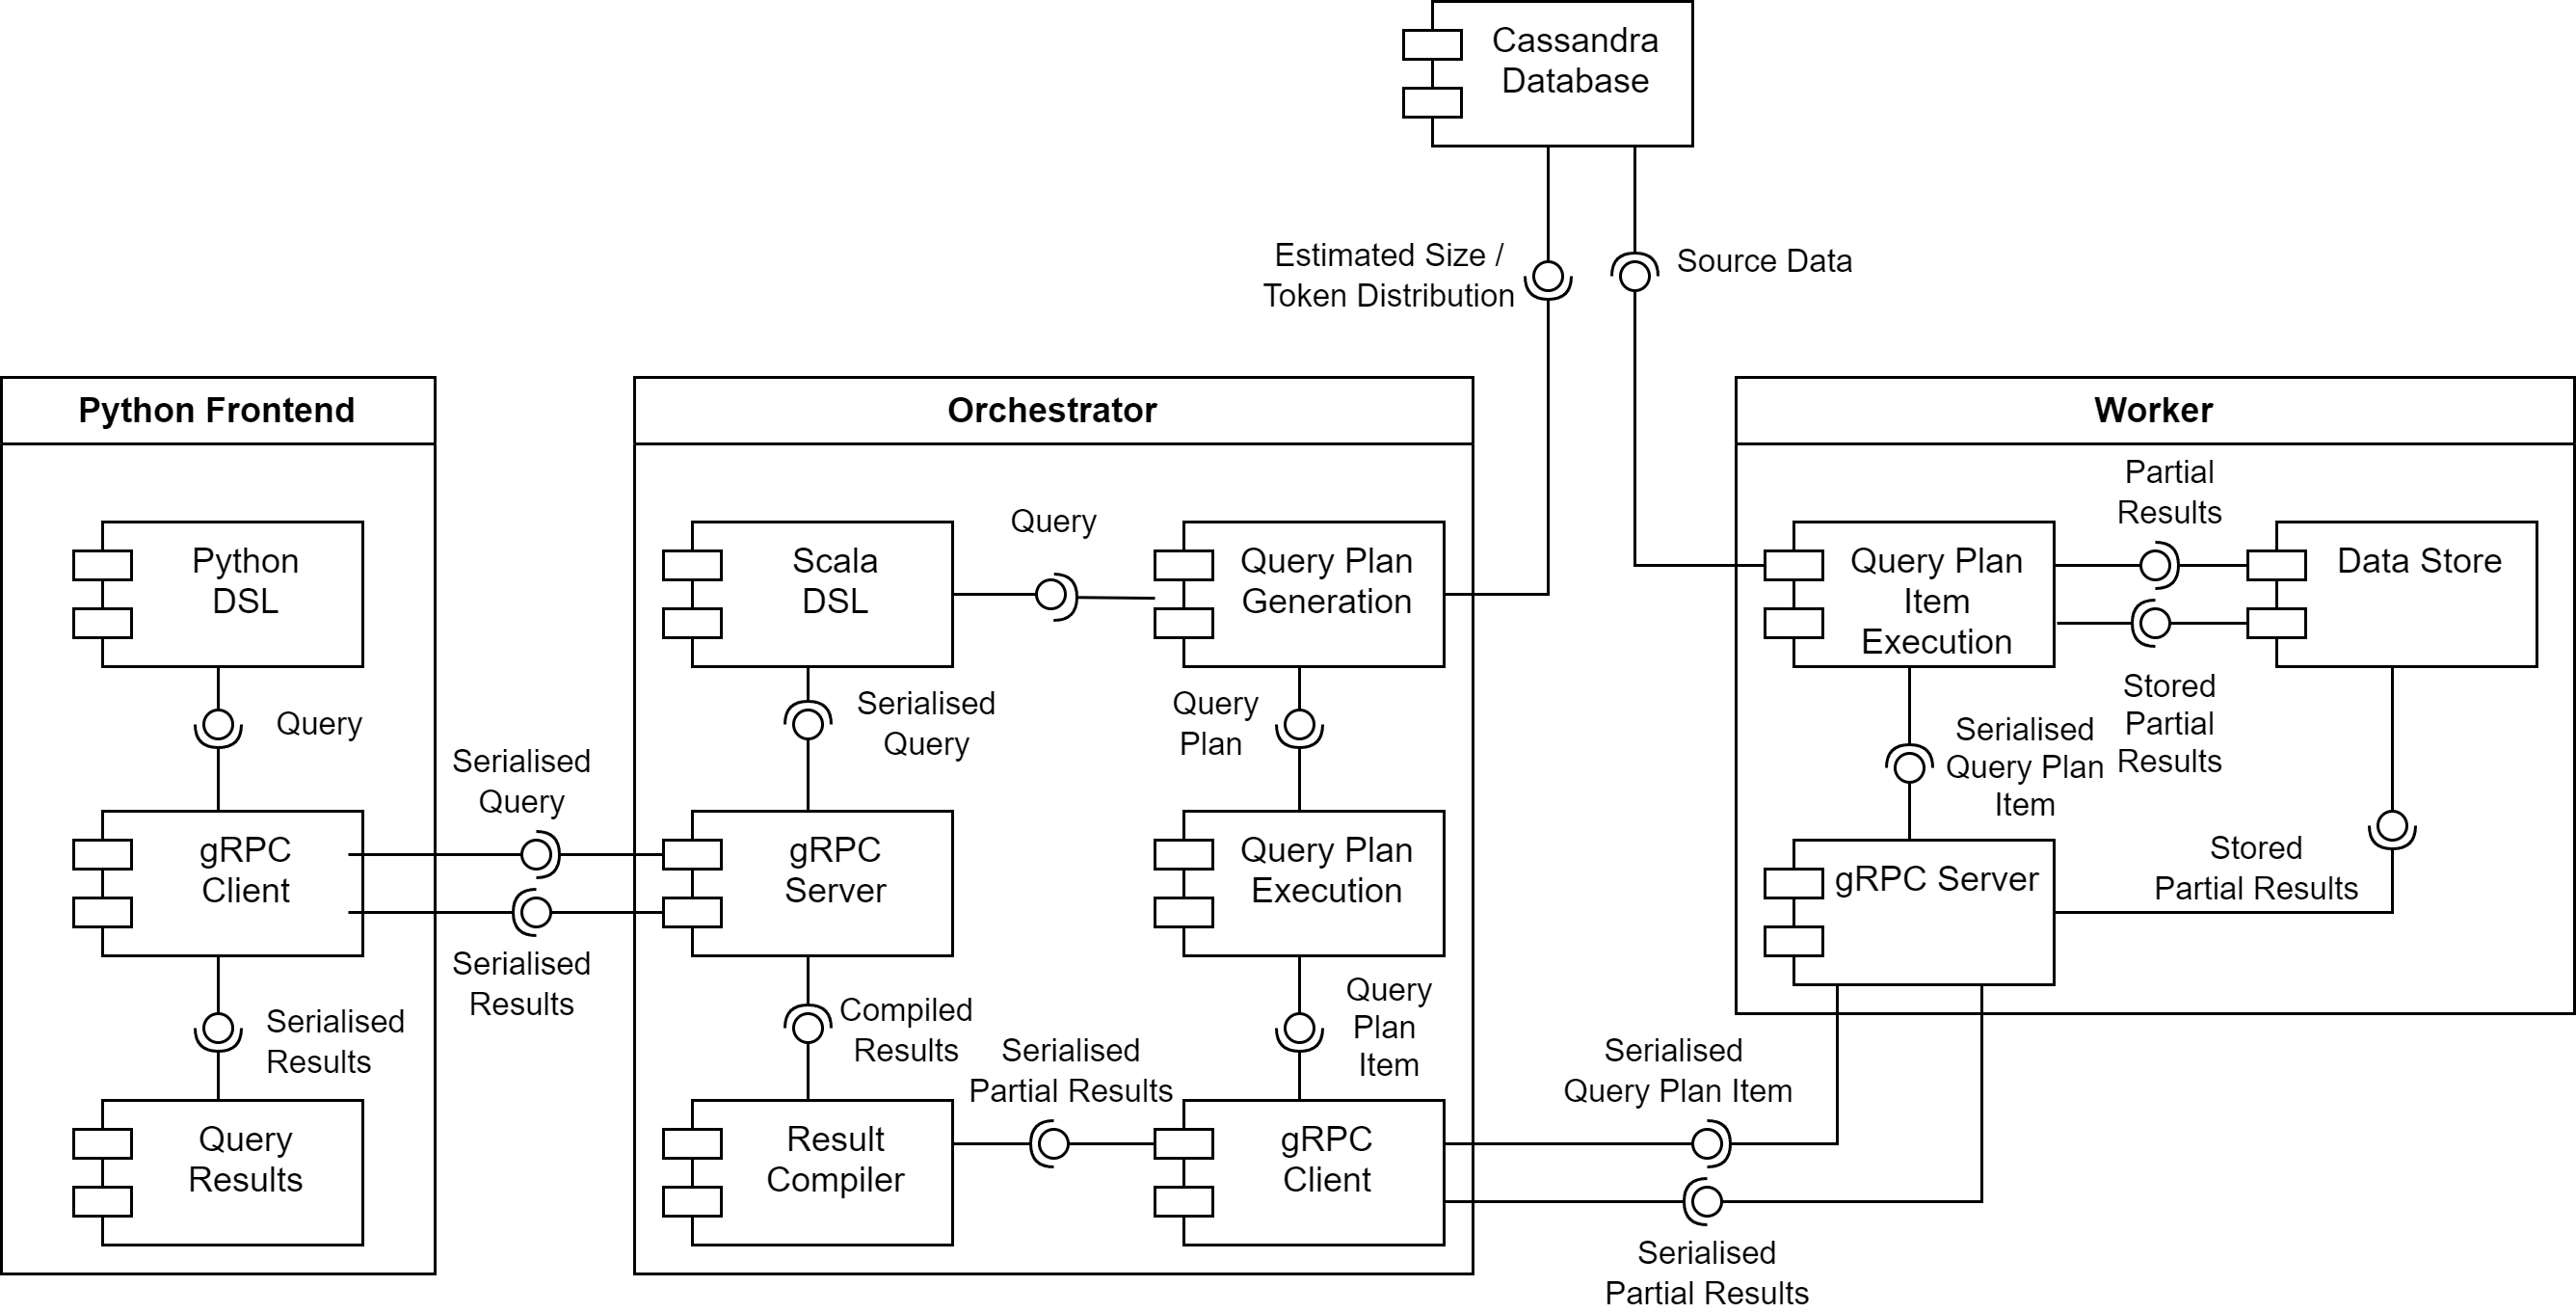
\includegraphics[width=0.7\textwidth]{chapters/diagrams/implementation/component-architecture-diagram}
	\caption{Solution Component Diagram}
	\label{fig:component-architecture-diagram}
\end{figure}

Figure \ref{fig:component-architecture-diagram} shows a component diagram for the core components, and their interactions. As described in Section \ref{sec:architecture}, the frontend is the user's entrypoint to the system. It acts as a terminal, allowing the user to define queries using the Python Domain Specific Language (DSL), and receive results. Queries are sent to the orchestrator, which acts as the central state management for the system. A number of components are used to get from query to result. First, it generates a query plan which describes the steps for computing a result. Then, the query plan is executed step-by-step, with the data used in each step being split up into a number of chunks of work (partitions) before being delegated to the workers. The workers are responsible for accepting these partitions, and performing the computation. Finally, when all query plan steps have been executed, the orchestrator fetches partial results from all workers, collates them into a final result, and returns this to the frontend. gRPC is used anywhere where network communication is required between the frontend, orchestrator and worker nodes.

The system supports three types of queries: Select, Filter and Group By. Both Select and Filter are row-level operations, meaning the workers do not have to pass data to one another during computation. However, Group By does need the workers to cross-communicate, which means they also require a temporary store to cache partial results.

\section{Type System}
\todo{Illustrative example - motivation: want to store table data, but need to know the type information of all values in the table}
\todo{Not super happy with this first sentence}
Any primitive value within the framework falls under the type system. Values can be combined into rows by storing multiple values in a list, and rows can be combined into tables by storing multiple rows in a list with a header. However, designing the interfaces to represent these values presents a challenge. Figure \ref{fig:type-system-motivation} demonstrates the problem. 

On the left, an example is shown where the raw data is held in lists. Type information cannot be used to determine the table's contents, as there are no shared types between the stored values. Therefore, to discover the type of a value, the system would have to perform runtime type checks against all supported types, adding a significant amount of overhead. 

On the right, a conceptual model is shown, using a lightweight container class. This holds the raw value, and the type information about the value at runtime, meaning that the system only needs to perform the runtime type check once in order to create the correct class instance. 

\begin{figure}[h]
	\centering
	% left - data stored in raw format - no information 
	% right - data stored in containers with value and type information, can infer what type the value is from the stored type information
	\caption{Type System - Motivating Example}
	\label{fig:type-system-motivation}
\end{figure}

Due to Java limitations, this conceptual solution is not entirely straightforward to implement. The container class could use a generic type parameter which stores the type information of the value inside the container. A row of data needs to support multiple types stored together, and this is not possible using generics as their type information is erased at runtime \cite{ghosh2004generics}. The container class could instead be defined as an interface, and each supported type provides an implementation of that interface, but this is not much better than the primitive type solution, as the runtime type check simply becomes a pattern match on the class instance. A solution that exploits some kind of polymorphism is preferred.

Scala provides a feature known as ClassTags \cite{scalaclasstags}. These saved the erased type information and also permit equality checks between ClassTag instances, meaning the framework can use the ClassTag to compare the type of a value to an expected type. This is used by \textit{FieldExpressions} to determine return types and function argument types; see Section \ref{subsec:fieldexpressions} for further information.

\todo{fix flow of these sections}
\subsection{Supported Types}
The type system supports a subset of Scala, Python, and Cassandra's types, shown in Figure \ref{fig:datatypes}.

\begin{figure}[h]
	\centering
	\begin{tabular}{| c | c | c | c |}
		\hline
		\textbf{Base Type} & \textbf{Python} & \textbf{Scala} & \textbf{Cassandra} \\ \hline
		Integer & int & Long & bigint \\ \hline
		Float & float & Double & double \\ \hline
		String & string & String & text \\ \hline
		Boolean & boolean & Boolean & boolean \\ \hline
		DateTime & datetime & Instant & timestamp \\ \hline
	\end{tabular}
	\caption{Primitive Types}
	\label{fig:datatypes}
\end{figure}

There were two main goals when selecting these primitive types. Firstly, every type should be able to be represented without data loss in all parts of the system. Secondly, it should be possible to represent the types in protobuf format, as this would allow for easy serialisation of result data. All types except DateTime can be converted to protobuf natively, and DateTimes are supported by serialising as an ISO8601 formatted string \cite{iso_8601}.

% does this flow
\subsection{ValueType Container Class}
The container class is defined using a base interface \textit{ValueType}, which captures the ClassTag requirement. This is used in both \textit{TableField}, which captures header field information (name and type), and \textit{TableValue}, which captures value information (value and type). By separating the ClassTag requirement from fields and values, \textit{TableFields} can be used to check the type of \textit{TableValues}, even though they hold different data. Concrete implementations for the 5 supported types are provided for both subclasses. Figure \ref{fig:type-system-hierarchy} shows the class hierarchy.

\begin{figure}[h]
	\centering
	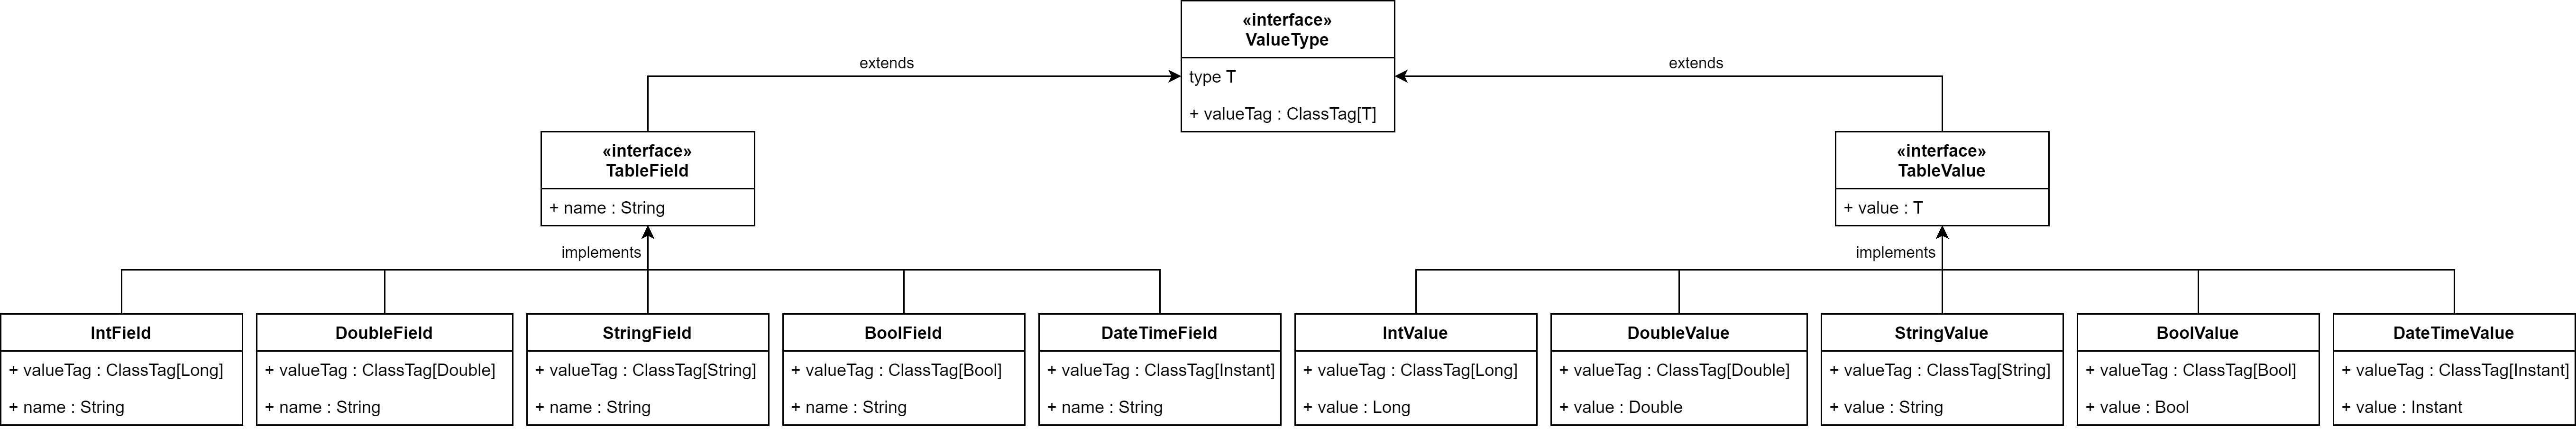
\includegraphics[width=0.7\textwidth]{chapters/diagrams/implementation/type-system-hierarchy}
	\caption{Custom Type System Hierarchy}
	\label{fig:type-system-hierarchy}
\end{figure}

\subsection{Result Model}
The hierarchy of classes and supported types provide everything needed to define the result of a computation, known as a \textit{TableResult}. Headers are defined as a sequence of \textit{TableFields} and result rows are stored as a two-dimensional array of \texttt{Option[TableValue]}. As defined in the requirements, null values must be supported, but the use of nulls in Scala is discouraged. Instead, Option is preferred as it is supported by all the typical functional methods. In this model, values are represented by \texttt{Some(TableValue())}, and null values are represented by \texttt{Nothing}. Figure \ref{fig:example-table-result} shows what an example result looks like using this definition.

\begin{figure}[h]
	\centering
	\begin{tabular}{l c  c  c l}
		\textbf{Header:} [ & IntField(\textcolor{deepgreen}{"ID"}),  & StringField(\textcolor{deepgreen}{"Name"}),  & BoolField(\textcolor{deepgreen}{"Passed"}) & ] \\
		\textbf{Row 1:} [[ & Some(IntValue(1)), & Some(StringValue(\textcolor{deepgreen}{"Alice"})), & Some(BoolValue(true)) & ], \\
		\textbf{Row 2:}  [ & Some(IntValue(2)), & None, & None & ], \\
		\textbf{Row 3:}  [ & Some(IntValue(3)), & Some(StringValue(\textcolor{deepgreen}{"Bob"})), & None & ]] \\
	\end{tabular}
	\caption{Example Table Result}
	\label{fig:example-table-result}
\end{figure}



\section{Domain Specific Language}
The user's interaction with the framework is driven entirely by the Domain Specific Language (DSL), which is modelled with SQL-like syntax. The language allows users to define expressions, then use these in computations like Select, Filter and Group By. Figure \ref{fig:dsl-high-level-example} provides a sample annotated DSL query, with links to the sections where each part is discussed.

\begin{figure}[ht]
	Initialise cluster connection and select a Cassandra source table:
	\begin{python}
ClusterManager("orchestrator-url")
  .cassandra_table("example", "table")
	\end{python}
	
	Select query, uses \textit{FieldExpressions} (Section \ref{subsec:fieldexpressions}) and Python Operators (Section \ref{subsec:dsl-python}):
	\begin{python}
  .select(
    F("id"),
    (F("duration") * 2).as_name("duration2"),
    Function.Left(Function.ToString(F("date")), 8)
      .as_name("yyyy-mm")
  )
	\end{python}

	Filter query, uses \textit{FieldComparisons} (Section \ref{subsec:fieldcomparisons}) and Python Operators (Section \ref{subsec:dsl-python}):
	\begin{python}
  .filter(
    (F("duration2") > 40) && 
  	(F("yyyy-mm").contains("2021")
  )
	\end{python}

	Group By query, uses \textit{AggregateExpressions} (Section \ref{subsec:aggregateexpressions}):
	\begin{python}
  .group_by(
    [F("duration2")],
    [
      Max(F("id")),
      Count(F("yyyy-mm"))
    ]
  )
	\end{python}
	\caption{Example DSL Query}
	\label{fig:dsl-high-level-example}
\end{figure}


\subsection{FieldExpressions}\label{subsec:fieldexpressions}
\textit{FieldExpressions} are a key part of the DSL, allowing the user to define arbitrary row-level calculations to be used as part of more complex operations. They are defined as an interface, with three subclasses:

\begin{itemize}
	\item Values: define literal values which never change across all rows
	\item Fields: when iterating over the rows of a result, gets the value from the named field in the current row.
	\item FunctionCalls: perform arbitrary function calls using further FieldExpressions as arguments.
\end{itemize}

Figure \ref{fig:field-expressions-examples} provides examples for each type of \textit{FieldExpression}.

\begin{figure}[ht]
	Values (from left to right): string "a", integer 1, double 1.5, boolean True, date 31/12/2021.
	\begin{python}
V("a") , V(1), V(1.5), V(True), V(datetime.date(2021, 12, 31))
	\end{python}

	Fields (from left to right): fieldName, duration, id, creationDate.
	\begin{python}
F("fieldName"), F("duration"), F("id"), F("creationDate")
	\end{python}

	Top Function: convert 'field1' to a string, then take the left 10 characters of each row.
	
	Bottom Function: multiply 'field2' by 2, then divide by "field3"
	\begin{python}
Function.Left(Function.ToString(F("field1")), 10)
(F("field2") * 2) / F("field3")
	\end{python}
	\caption{\textit{FieldExpression} implementations and examples}
	\label{fig:field-expressions-examples}
\end{figure}

Many basic functions have been implemented, including arithmetic, string and cast operations. ver, the function system is designed to be extensible. A number of helper classes are defined to allow the creation of basic unary, binary and ternary functions, but \textit{FunctionCall} is itself an interface which can be given completely custom implementations if required. The main constraint on the functions that can be defined are that only the 5 primitive input types are supported.

\paragraph{Type Resolution} 
Type Resolution on FieldExpressions is performed in two stages: a resolution step, and an evaluation step. The resolution step takes in type information from the header of the input result, and verifies that the \textit{FieldExpression} is well typed with regards to that result. This is required for Fields, which can be valid for one result but invalid for another if the field name is not present in the result header; Figure \ref{fig:field-type-resolution} shows an example of this. The evaluation step performs the computation on a row from that result without any type checking. \todo{edit this to include this example, and an example of a function being invalid if the type of the field is wrong}

\begin{figure}[ht]
	\centering
	\subfloat[\centering Valid - able to evaluate this result]{
		\begin{tabular}{l c l}
			\textbf{Header:} [& IntField(\textcolor{deepgreen}{"field"}) ] \\
		\end{tabular}
	}
	\qquad
	\subfloat[\centering Invalid - unable to evaluate this result]{
		\begin{tabular}{l c l}
			\textbf{Header:} [& StringField(\textcolor{deepgreen}{"differentField"}) ] \\
		\end{tabular}
	}
	
	\caption{Type Resolution of F(\textcolor{deepgreen}{"field"})}
	\label{fig:field-type-resolution}
\end{figure}

This two-step process has a number of benefits. The resolution step enables a form of polymorphism on some functions like arithmetic operations. These functions determine what types are returned by their sub-expressions during resolution, and resolve to the correct version for evaluation. For example, the add function can resolve to \textit{AddInt}, \textit{AddDouble}, or \textit{Concat}. This reduces the overhead at runtime as type checking does not need to be performed for each row when making a function call. Unchecked casts are used here instead, demonstrated for a binary function in Figure \ref{fig:fieldexpression-unchecked-casts}
	
\begin{figure}[ht]
	\centering
	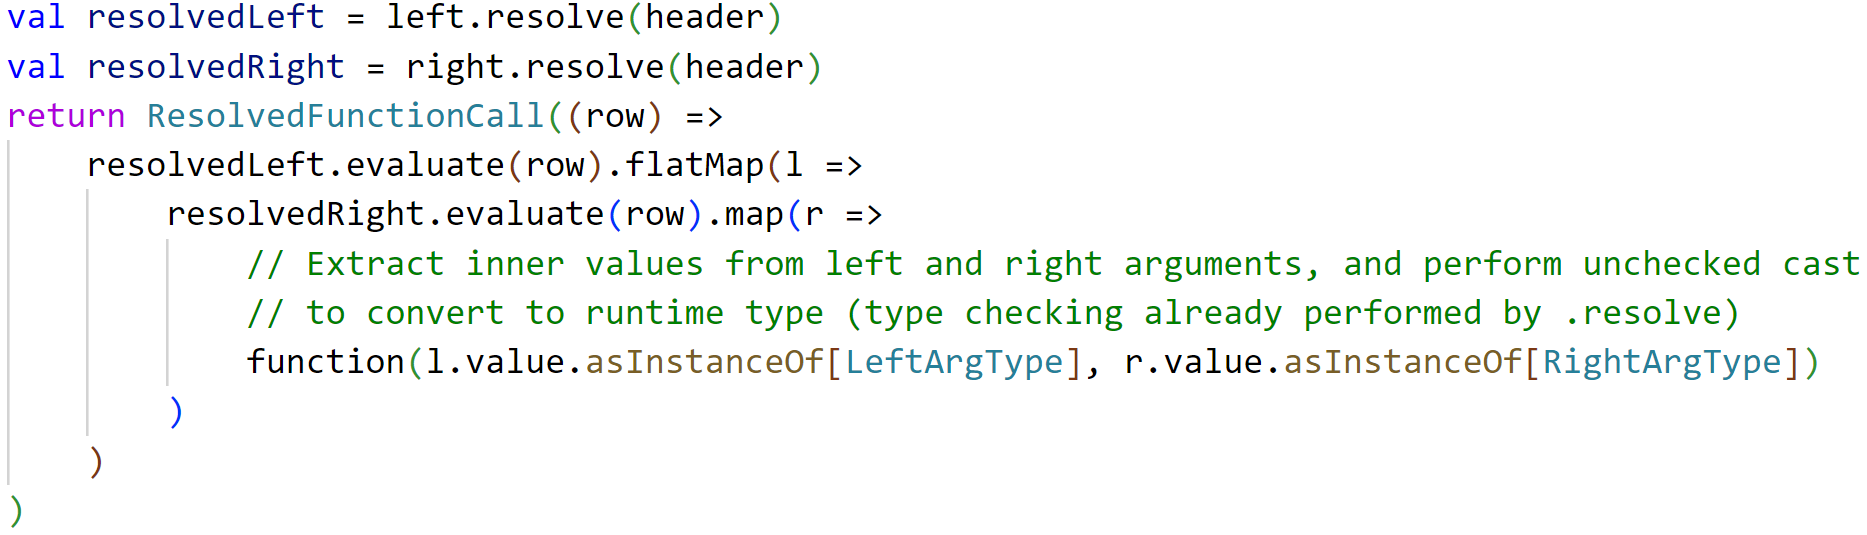
\includegraphics[width=\textwidth]{chapters/diagrams/implementation/type-resolution-unchecked-casts}
	\caption{Runtime Evaluation of Functions}
	\label{fig:fieldexpression-unchecked-casts}
\end{figure}


\paragraph{Named Expressions}
When performing a Select operation, the output fields are all expected to be named. This allows the user to chain operations by referencing fields from the previous input. Figure \ref{fig:namedfieldexpression-examples} shows the two ways of naming a field: \textit{FieldExpressions} can be assigned a user-defined name, or \textit{F()} expressions will also keep their name automatically.

\begin{figure}[ht]
	Top Expression Name: 'twice\textunderscore duration'
	
	Bottom Expression Name: 'creation\textunderscore date'
	\begin{python}
(F("duration") * 2).as_name("twice_duration")
F("creation_date")
	\end{python}
	\caption{\textit{NamedFieldExpression} examples}
	\label{fig:namedfieldexpression-examples}
\end{figure}

\subsection{FieldComparisons}\label{subsec:fieldcomparisons}
\textit{FieldComparisons} are another key building block of the DSL, allowing the user to define arbitrary row-level comparisons. \textit{FieldComparisons} use a two-step resolution-evaluation process to accommodate the same process as \textit{FieldExpressions}. They are defined as an interface, with a number of comparison types implemented already, including null, equality, numerical and string comparisons. Examples of each are shown in Figure \ref{fig:field-comparisons-examples}.

\begin{figure}[htp]
	Null checks: verify whether an expression is null or not null.
	\begin{python}
F("duration").is_null()
F("duration").is_not_null()
	\end{python}
	
	Equality checks: verify whether two \textit{FieldExpressions} are equal or not equal. 
	\begin{python}
F("duration") == 20
F("duration") != F("other_duration")
	\end{python}

	Ordering checks: apply ordered comparators between two \textit{FieldExpressions}.
	\begin{python}
F("duration") < 20
F("duration") <= 19
F("duration") > 20
F("duration") >= 21
	\end{python}

	String checks: apply contains, starts with and ends with operators (case insensitive versions also available).
	\begin{python}
F("name").contains("Alice")
F("name").starts_with("Bob")
F("name").ends_with("Smith")
	\end{python}
	\caption{\textit{FieldComparison} examples}
	\label{fig:field-comparisons-examples}
\end{figure}

\paragraph{Combined Comparisons}
The user is able to combine multiple FieldComparisons using AND/OR operators, shown in Figure \ref{fig:field-comparisons-combiners}. This is a lightweight wrapper around Scala's own AND (\texttt{\&\&}) and OR (\texttt{||}) boolean operators, meaning optimisations like short circuiting operate as normal.

\begin{figure}[htp]
	\begin{python}
(F("duration") < 20) && (F("name").starts_with("Bob"))
(F("duration") < 20) || (F("name").starts_with("Bob"))
(F("duration") < 20) && (
  (F("name").contains("Bob")) || (F("name").contains("Alice"))
)
	\end{python}
	\caption{\textit{FieldComparison} AND/OR Combinations}
	\label{fig:field-comparisons-combiners}
\end{figure}

\subsection{Aggregate Expressions}\label{subsec:aggregateexpressions}
\textit{AggregateExpressions} are the final part of the DSL. These are used only as part of Group Bys, and allow the user to define methods of aggregating all rows of a result. They take a \textit{NamedFieldExpression} as an argument, and compute a single row output from any number of input result rows.

The supported operations are Minimum, Maximum, Sum, Average, Count, and String Concatenation, and they are polymorphic where possible. For example, minimum and maximum handle numeric types by ordering numerically and string types lexicographically. Figure \ref{fig:aggregate-expressions-examples} shows examples of \textit{AggregateExpressions}.

\begin{figure}[htp]
	\begin{python}
Max(Function.ToString(F("date")).as_name("date_string"))
Max(F("duration"))
Sum(F("amount"))
Count(F("id"))
	\end{python}
	\caption{\textit{AggregateExpression} examples}
	\label{fig:aggregate-expressions-examples}
\end{figure}

\subsection{Protocol Buffer Serialisation}
All components of the DSL have been designed to be serialised to protobuf format. This allows any queries written by the user to be passed around the system using gRPC, and if required the query can also be serialised to a file. The results of a query are also serialisable, to allow the system to return query results to the user. gRPC has a size limit of 4MB for individual messages, so results are split up by row and streamed individually.

\subsection{Python Implementation}\label{subsec:dsl-python}
The Python frontend is designed to be straightforward to use, hiding the complexities of the computation being performed in the backend. A number of Python-specific features were used to help with this.

Python allows developers to override common operators, including arithmetic and comparison, with custom definitions. The Python implementation of \textit{FieldExpression} overrides the arithmetic operators, as well as comparison operators to allow the user to automatically generate functions and \textit{FieldComparisons}, without having to write the full definition.

Furthermore, as discussed in \ref{subsec:frontend-design}, pandas is widely used for data analysis in Python \cite{reback2020pandas}. The frontend is able to convert query results from their protobuf definition to a pandas DataFrame to allow further analysis to be performed immediately.



\section{Data Model}\label{subsec:data-model}
% This section should be clear and understandable, as much of the rest refers to partial and full versions
The data model is split into two key components: \textit{DataSource} and \textit{Table}. 

\textit{DataSource} is an interface, representing any part of the query where data must be rearranged into new partitions, including Cassandra source data, and Group By operations. \textit{Table} is a class, representing any part of the query containing purely row-level computations, including Select and Filter operations. It is composed of a \textit{DataSource} and a list of row-level computations known as \textit{TableTransformations}. To compute its output, the \textit{DataSource} is computed first, then all transformations are applied sequentially.

Optionally, \textit{DataSources} can have dependent \textit{Tables} which must be calculated first. For example, a Group By \textit{DataSource} requires a single \textit{Table} to be fully computed before it can be generated. A Cassandra \textit{DataSource} will always act as the terminal component for a query, as it has no dependencies.

For demonstration purposes, Figure \ref{fig:filter-select-query} shows a Filter and Select query in the DSL, and the data model. Note that any number of Select and Filter operations can be placed in the Table component, as no new partitions are required to produce the result.

\begin{figure}[htp]
	\centering
	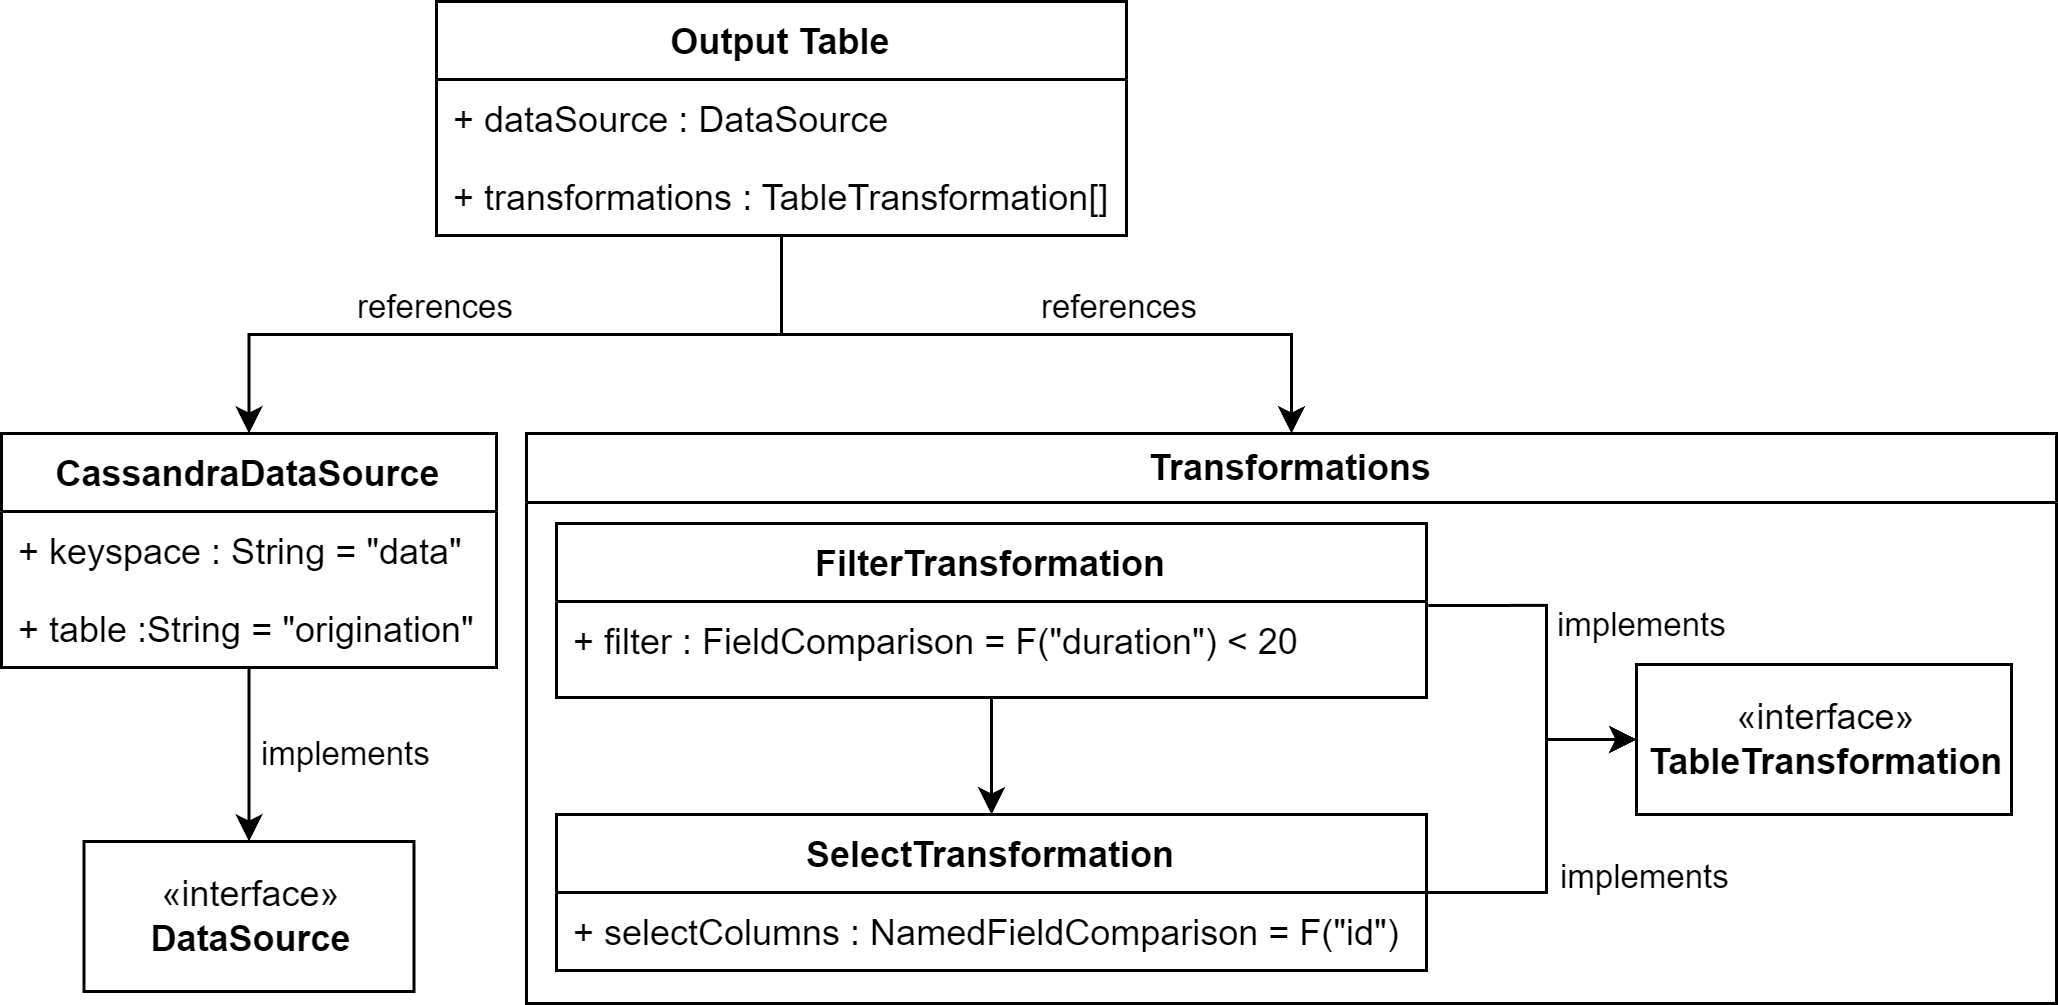
\includegraphics[width=0.8\textwidth]{chapters/diagrams/implementation/filter-select-query}
	\begin{python}
ClusterManager("orchestrator-service")
.cassandra_table("data", "origination")
.filter(F("duration") < 20)
.select(F("id"))
.evaluate()
	\end{python}
	\caption{Example Filter and Select Query}
	\label{fig:filter-select-query}
\end{figure}


Figure \ref{fig:group-by-query} shows a more complex query containing a Group By in the DSL, and the data model. The dependent table (bottom left) is calculated first, and its output is used to compute the Group By, in \textit{GroupByDataSource}. The final output is then generated in the output table.

\begin{figure}[htp]
	\centering
	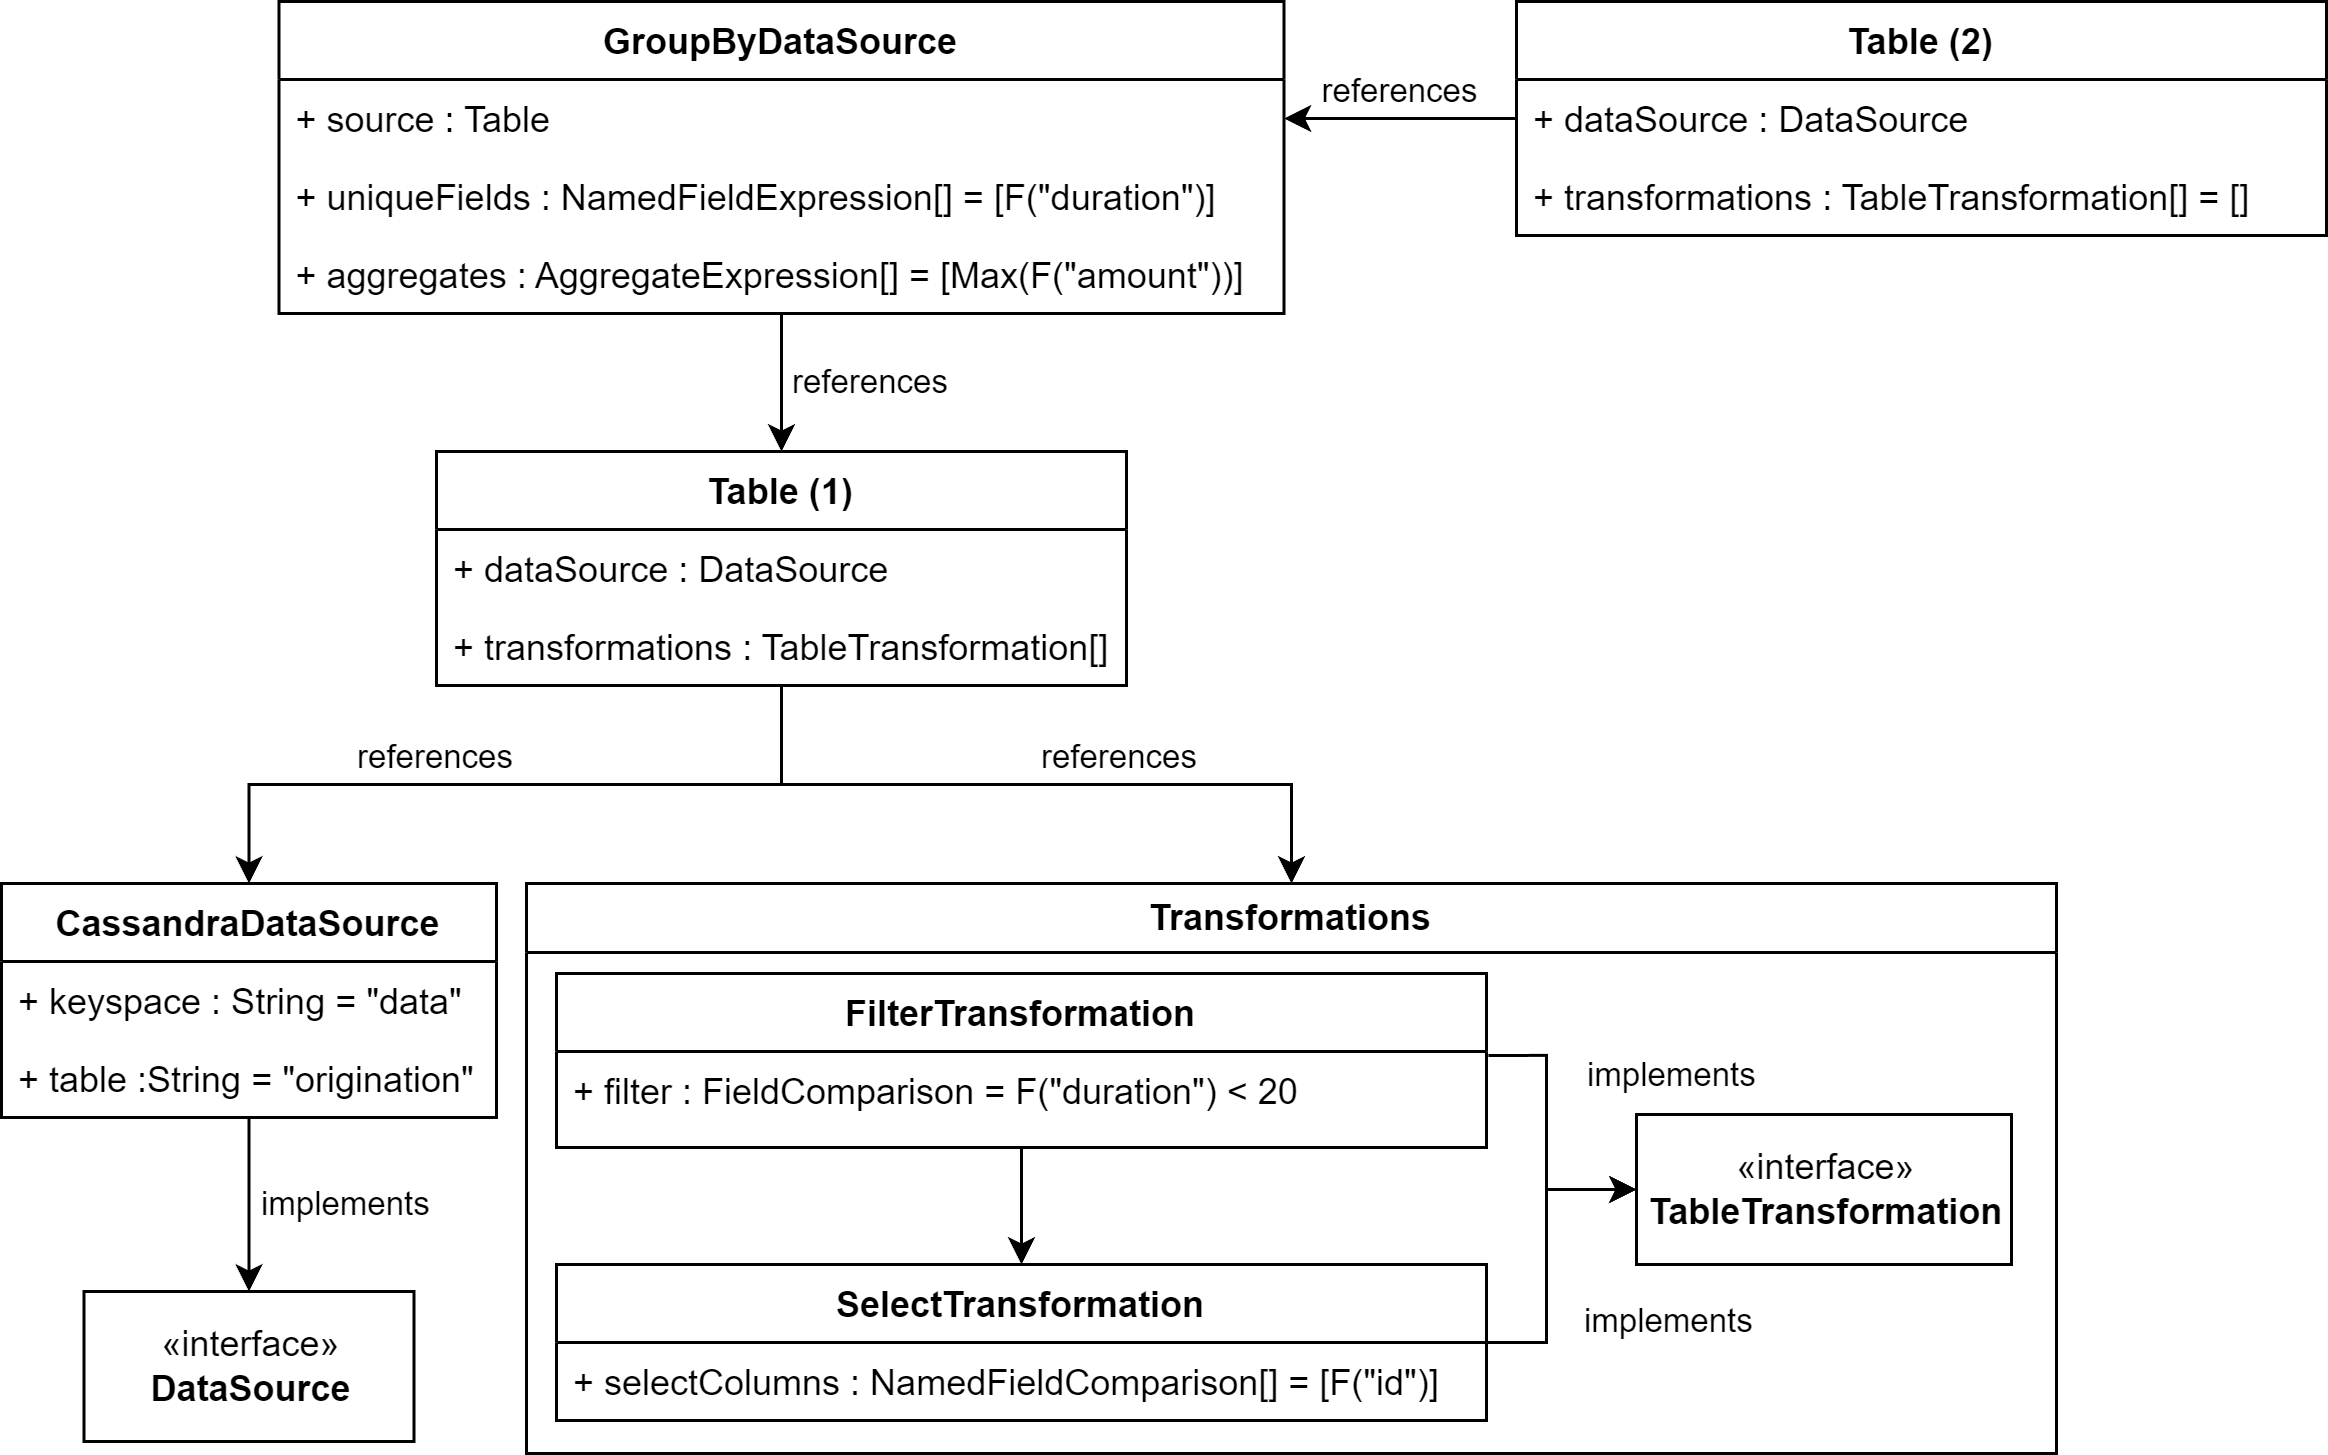
\includegraphics[width=0.8\textwidth]{chapters/diagrams/implementation/group-by-query}
	\linebreak
	\begin{python}
ClusterManager("orchestrator-service")
.cassandra_table("data", "origination")
.filter(F("duration") < 20)
.select(F("id"))
.group_by([F("duration")], [Max(F("amount"))])
.evaluate()
	\end{python}
	\caption{Example Group By Query}
	\label{fig:group-by-query}
\end{figure}

A \textit{Table} or \textit{DataSource} cannot be computed directly, but must first be split into partitions, which are provided by the \textit{DataSource}. These partitions are represented by the interface \textit{PartialDataSource}, with the partitioning method being specific to each implementation. The \textit{Table} class has a similar partial form, \textit{PartialTable}, which references a \textit{PartialDataSource} and can be computed directly. Both \textit{PartialDataSource} and \textit{PartialTable} always hold a reference to the complete version of themselves. To demonstrate how to produce a final result from a set of partial results, Figure \ref{fig:partial-filter-select-query} shows a high level example of one possible way of partitioning and computing the previous Filter and Select query.

\begin{figure}[h]
	\centering
	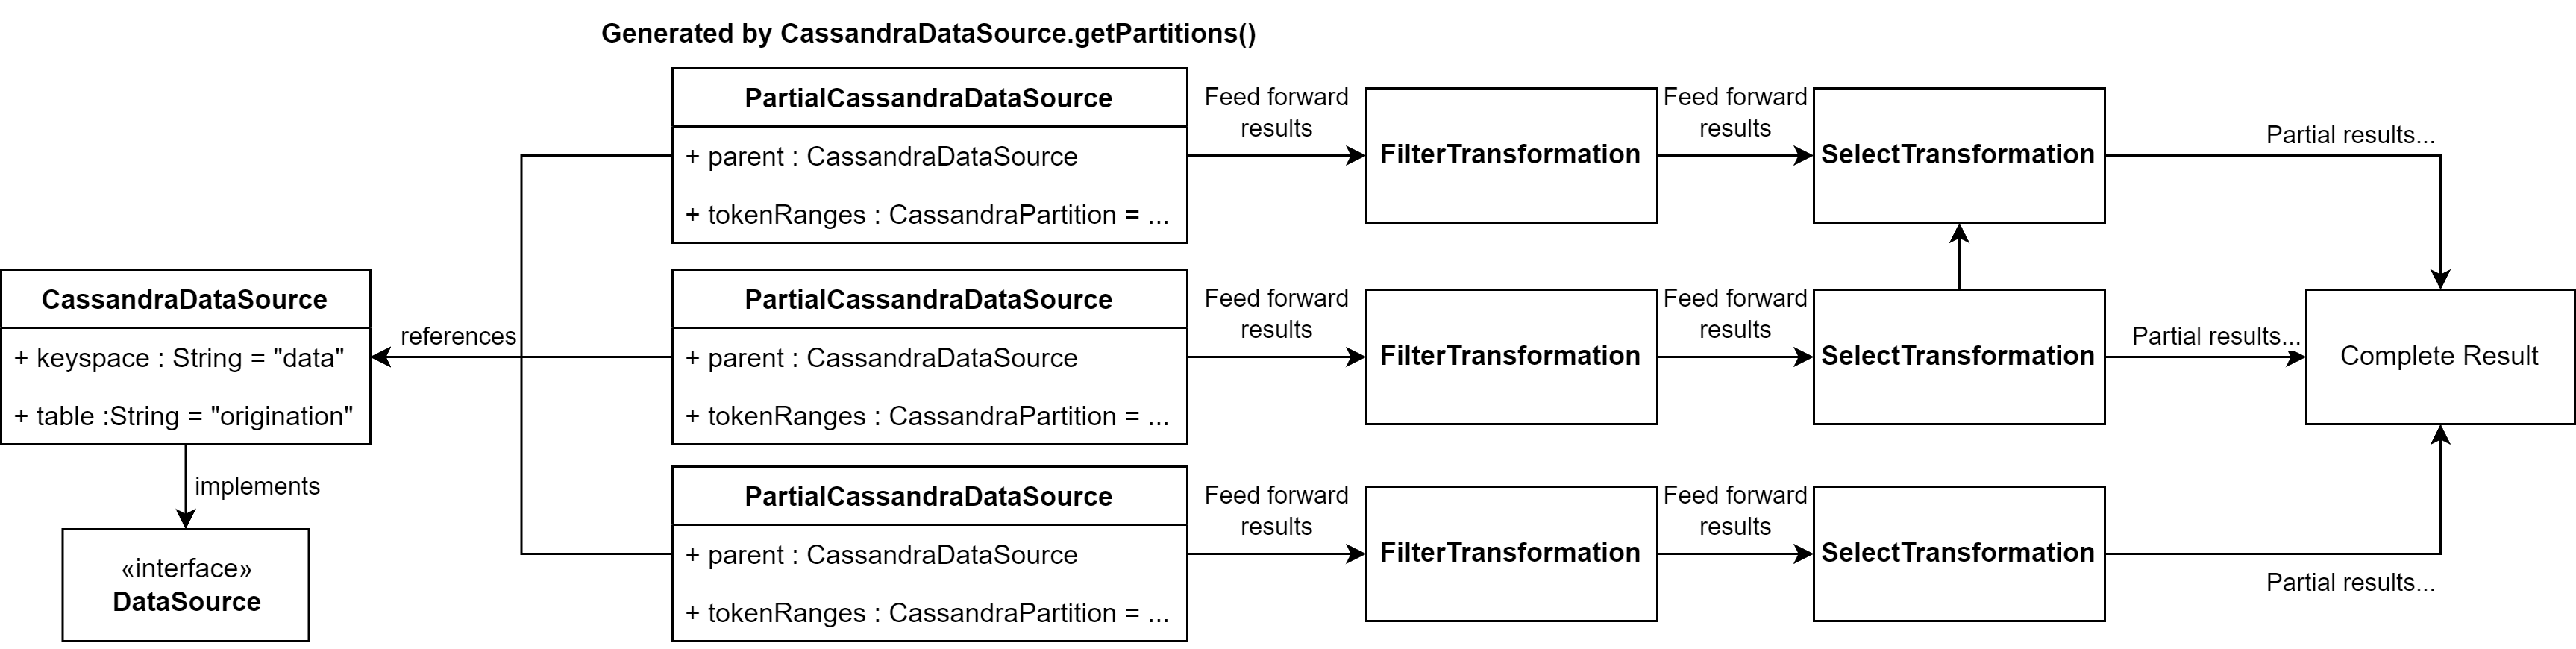
\includegraphics[width=\textwidth]{chapters/diagrams/implementation/partial-filter-select-query}
	\caption{Example Filter and Select Query}
	\label{fig:partial-filter-select-query}
\end{figure}



\section{Data Store}
The data store is the most important component for the worker implementation. It allows the workers to store partially computed data, which can be reused in later parts of the query execution. In particular when workers are communicating with one another, it is likely that the worker will be processing more than one request at the same time, which presents issues with handling concurrency and synchronisation.

The approach taken to solve this uses the actor model, first introduced in 1973 by Carl Hewitt \cite{hewitt1973session}. Specifically, the Akka Actors framework was chosen as an implementation of the actor model in Scala \cite{akkaactors}. The actor model abstracts away the complexity of synchronisation and thread management. Instead, components of the system become actors. Each actor defines a set of messages that it accepts, and the response to each message, and the framework provides a guarantee that an actor will only ever process one message at a time.

The data store is modelled as an actor which stores results as key-value pairs. Three kinds of data can be used as keys for storage: \textit{Table} computation results, \textit{DataSource} computation results and hashed data results, which are used in the process of computing a Group By partition. 

For each supported type of data, the data store uses a two-stage lookup, internally implemented using nested HashMaps. First, the full version of the data (\textit{Table} or \textit{DataSource}) is looked up, then the partial version (\textit{PartialTable} or \textit{PartialDataSource}). Partial forms of \textit{Tables} and \textit{DataSources} always contain a reference to the full version, but not the other way around. Therefore, this decision does not increase the time taken to insert new data significantly, but it is particularly useful when fetching the results for a \textit{Table}, or removing a \textit{Table} or \textit{DataSource}. Without this approach, completing these operations would require searching the entire Map to find any matches, turning the O(1) lookup time into O(n).

\subsection{Spill to Memory}
In situations with very large datasets, the amount of memory available to the workers will be less than the amount of data the system attempts to load. In this case, it is likely that the JVM will run out of heap space, causing a crash when it attempts to allocate more memory to store data. Therefore, the system features a module which allows it to move cached data onto disk to free up heap space. This module is part of the data store, and functions transparently to the rest of the system - data store queries are the same whether the result is held in-memory or on-disk.

\paragraph{Storage Interface}
To implement the spill process, an interface \textit{StoredTableResult} is defined. This interface holds a key which corresponds to that result, and a \textit{get} operation to retrieve the result data. There are two main subclasses that implement this interface: \textit{InMemoryTableResult} and \textit{ProtobufTableResult}. 

\textit{InMemoryTableResult} is a simple wrapper for the interface, which simply contains the result and holds it in memory. It also features a \textit{spillToDisk} method which moves the data onto disk by creating a file under a randomised folder name for that execution, with the name set to the hashcode of the key. 

\textit{ProtobufTableResult} only holds a pointer to the data on disk, and reads the data from there when the \textit{get} operation is called. It also features a cleanup method which removes the stored data from disk.

\paragraph{Spill Process}
The data store is responsible for managing in-memory and on-disk data. Before almost every operation on the data store, it makes a check for the current memory utilisation, which is calculated using a set of methods on the \textit{Runtime} class \cite{javaruntimeclass}. If the memory utilisation is over a given threshold, the data store attempts to spill at least the amount of bytes over the utilisation threshold. 

Figure \ref{fig:bytes-over-memory-threshold} shows how the amount of bytes over a percentage threshold is calculated. The division on the left calculates the current memory utilisation percentage, then the threshold is subtracted to get the percentage amount over it. This is multiplied by the total number of bytes to get the number of bytes that the percentage represents.

\begin{figure}[h]
	\centering
	\[ \left( \frac{\text{Bytes in Use}}{\text{Total Bytes Available}} - \text{Threshold} \right) * \text{Total Bytes Available} \]
	\caption{Number of Bytes Over Memory Threshold}
	\label{fig:bytes-over-memory-threshold}
\end{figure}

To perform the spill, the data store will follow the decision tree shown in Figure \ref{fig:spill-to-disk-process} After the process is completed, the data store forces the JVM to perform Garbage Collection to immediately free the relevant amount of memory.

\begin{figure}[h]
	\centering
	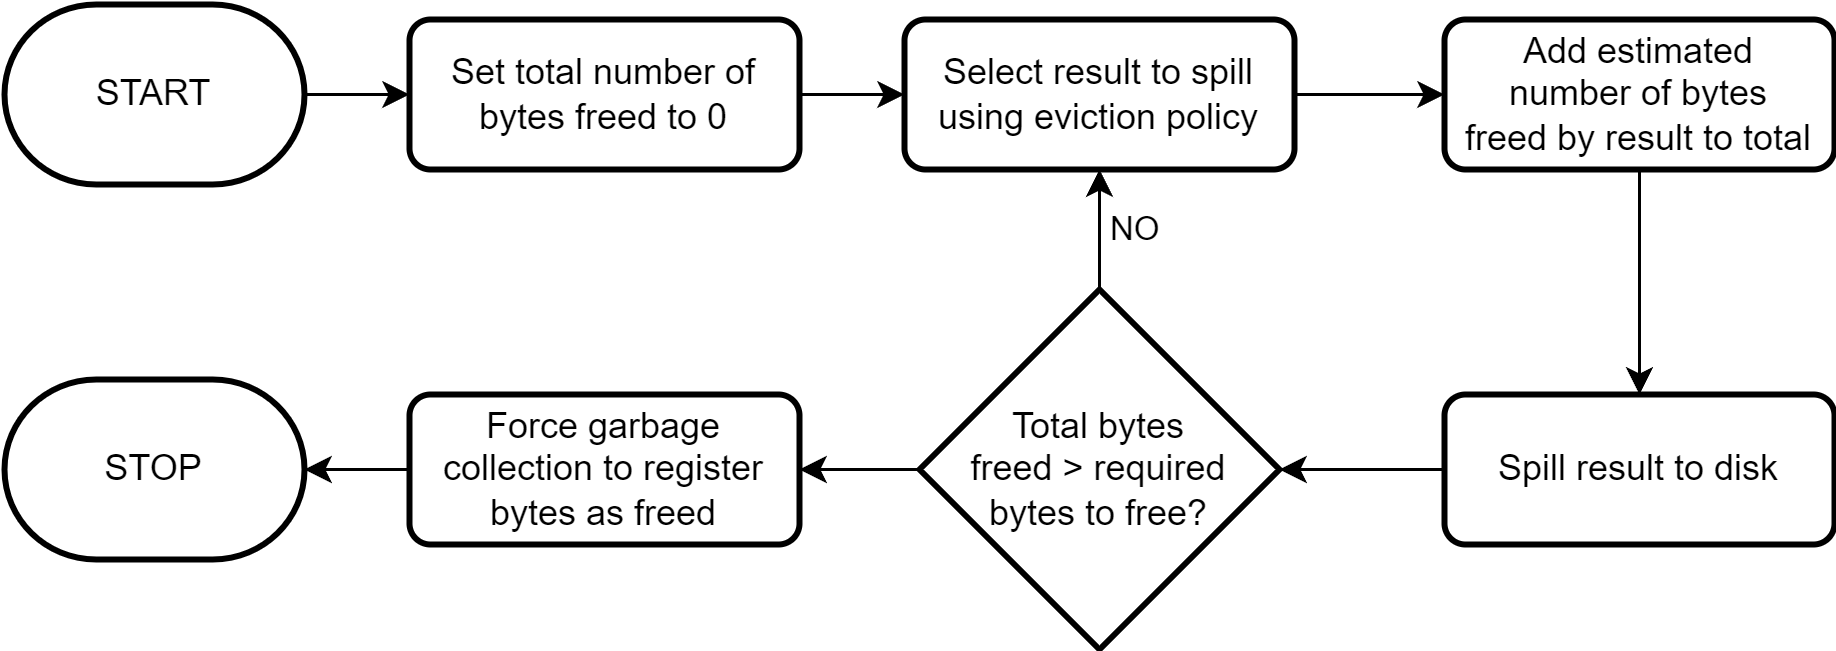
\includegraphics[width=0.6\textwidth]{chapters/diagrams/implementation/spill-to-disk-process}
	\caption{Spill to Disk Decision Tree}
	\label{fig:spill-to-disk-process}
\end{figure}

This process is not without flaws. It relies on no other class in the current JVM instance holding references to any of the results being spilled. In the controlled worker environment, it is possible to ensure this is the case, meaning the spill works reliably, but this approach would not work more generally. Also, this approach is reliant on size estimates, meaning the actual amount of memory freed will not be the same as the estimated memory freed. With a suitably low threshold for spilling (60-70\% of maximum memory) and regular checks of memory utilisation, this risk does not become a real problem.

\paragraph{Eviction Policy}
Finally, the policy for determining results to spill is important. A policy that does not fit the way the results are being used could result in large performance impacts, as it could cause antipatterns like the data store spilling a result, then immediately reading it back to memory.

The data store makes use of a least-recently-used (LRU) policy to determine the next result to spill to disk, implemented using an ordered list containing all in-memory results. When results are inserted into the data store, they are added to the end of the list. When results are read from the data store, they are moved to the end of the list. Then, when a result must be selected for spill, the item at the head of the list is chosen and removed.



\section{Partitioning}
One of the most important jobs of the orchestrator during a computation is to calculate partitions. There are two situations where partitions need to be calculated: when pulling source data from Cassandra, and when computing a Group By. The overall goal is to split the dataset into roughly equal chunks of a manageable size. 

\subsection{Cassandra}
As described in the Design Chapter, Cassandra was selected as the persistent storage module because its storage model closely matches the type of partitioning the system requires. The Cassandra \textit{DataSource} getPartitions method investigates the source data in the database, and generates an appropriate number of partitions. This process is described below.

When data is stored in Cassandra, the primary key of each row already has a 64-bit token assigned to it. Cassandra allows queries to filter on ranges of these tokens, meaning the data can be split up and read from the database in chunks. To be able to ensure the partitions are a manageable, defined size, an estimate of the size of the full source data is required. Cassandra provides this information in the \texttt{system.size\char`_estimates} table. This table provides an estimate of the size of each table in the database, and these are generated automatically every 5 minutes.

From a size estimate of the full table, estimates can be calculated for any given token range using the equation in Figure \ref{fig:token-range-estimation}. The fraction calculates the percentage of all tokens that the given token range represents.

\begin{figure}[h]
	\centering
	\[ \frac{\text{Number of Tokens in Token Range}}{\text{Total Number of Tokens: } ((2^{63}-1) - (-2^{63}))} \times \text{Estimated Table Size} \]
	\caption{Token Range Size Estimation Equation}
	\label{fig:token-range-estimation}
\end{figure}

Using this equation, it first gathers the token ranges which each node is responsible for storing. Then, it performs a joining and splitting process over each node, depending on the size of the token ranges. The set of token ranges produced after this process are the partitions used during the computation. The flowchart in Figure \ref{fig:cassandra-partitioning-decision-tree} shows the full process for generating the output partitions, 

\begin{figure}[h]
	\centering
	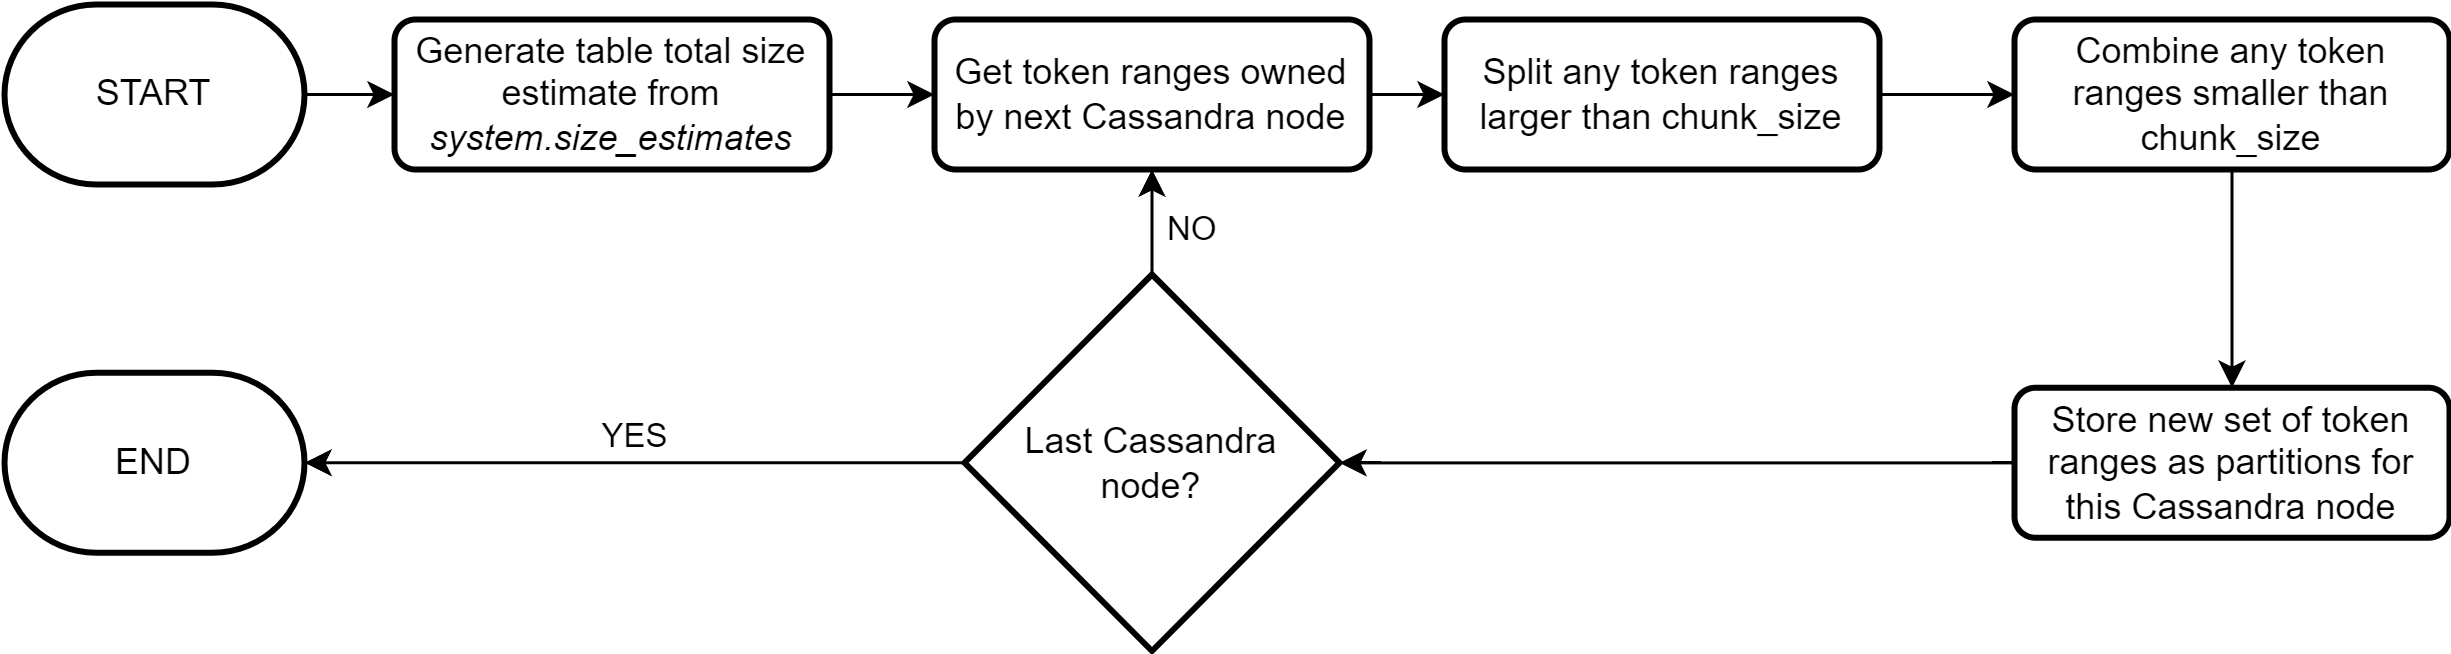
\includegraphics[width=0.8\textwidth]{chapters/diagrams/implementation/cassandra-partitioning-decision-tree}
	\caption{Cassandra Partitioning Process}
	\label{fig:cassandra-partitioning-decision-tree}
\end{figure}


Figure \ref{fig:cassandra-split-process} demonstrates how the splitting process works. The system calculates how much times larger the token range currently is than the goal partition size, then divides the token range evenly by that amount.

\begin{figure}[h]
	\centering
	\subfloat[\centering Equation]{\raisebox{1.5cm}{$ \text{Number of Splits} = \frac{\text{Token Range Size}}{\text{Chunk Size}} $}}
	\qquad
	\subfloat[\centering Example]{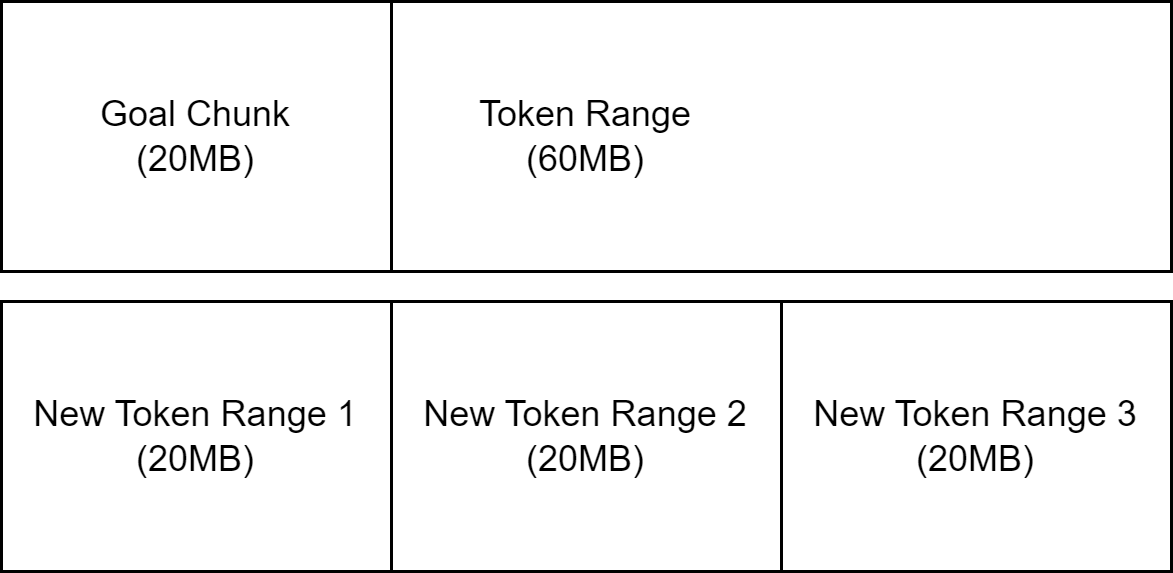
\includegraphics[width=0.4\textwidth]{chapters/diagrams/implementation/cassandra-split-example}}
	\caption{Token Range Splitting}
	\label{fig:cassandra-split-process}
\end{figure}

Figure \ref{fig:cassandra-join-process} provides an example how the joining process works. Given a sorted list of token ranges, the system repeatedly adds sequential elements to a partition until it is larger than the goal partition size. Then, the partition is marked as completed. The list is sorted by size ascending to ensure the smallest number of partitions are created - if there are a large number of very small token ranges, these will be combined into a single large partition together.

\begin{figure}[h]
	\centering
	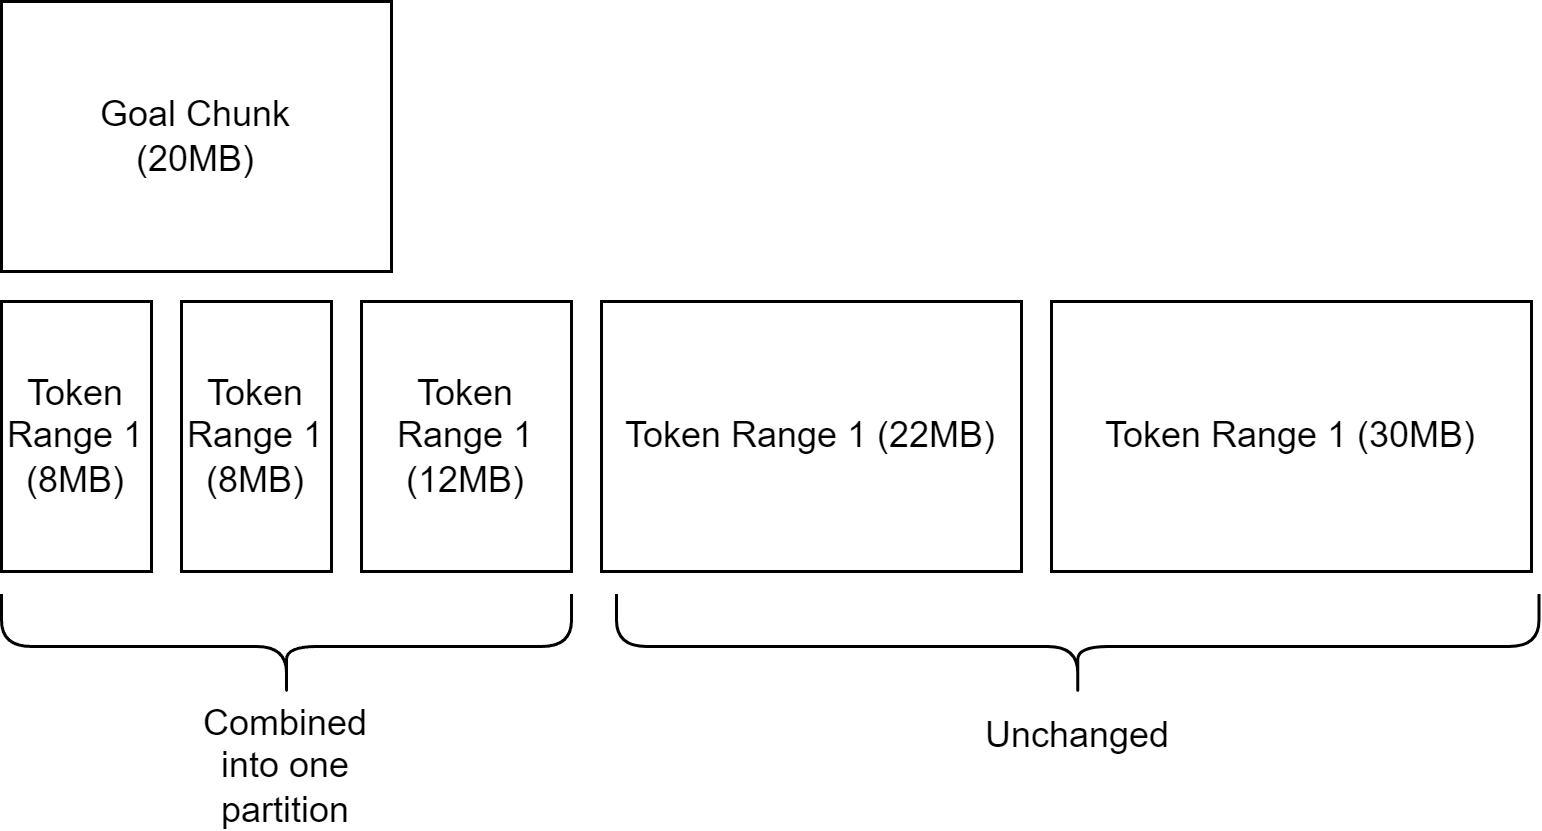
\includegraphics[width=0.5\textwidth]{chapters/diagrams/implementation/cassandra-join-example}
	\caption{Token Range Joining Example}
	\label{fig:cassandra-join-process}
\end{figure}

The Cassandra Java Driver provides a wide range of helper functions for performing the joining and splitting of token ranges accurately to produce new token ranges. The system simply calculates how much joining or splitting is required based on the size of the token ranges and the table size estimate. It then uses the driver to perform the calculations.

\subsection{Cassandra Data Co-Location}\label{subsec:colocation}
Once the list of partitions for each Cassandra node are generated, the system attempts to co-locate workers to Cassandra nodes. The goal of this process is to produce an \textit{optimal assignment} of partitions, where each partition is matched to one or more workers to minimise network latency when fetching the data from Cassandra.

To do this, each worker first calculates its closest Cassandra node. This is done by opening a TCP connection multiple times with each Cassandra node, and averaging the time taken over multiple attempts. The node with the lowest average latency is selected as the closest node. The orchestrator uses this information to match each worker to a Cassandra node and its corresponding list of partitions. The output is an optimal assignment between workers and partitions. It is possible for more than one worker to be matched to the same set of partitions, and it is also possible for a set of partitions to have no co-located worker nodes. In this case, they are kept as unassigned, and the work assignment algorithm handles their allocation. Figure \ref{fig:optimal-assignment-example} shows an example cluster setup with three physical nodes, and the optimal assignment after this process is complete.

\begin{figure}[h]
	\centering
	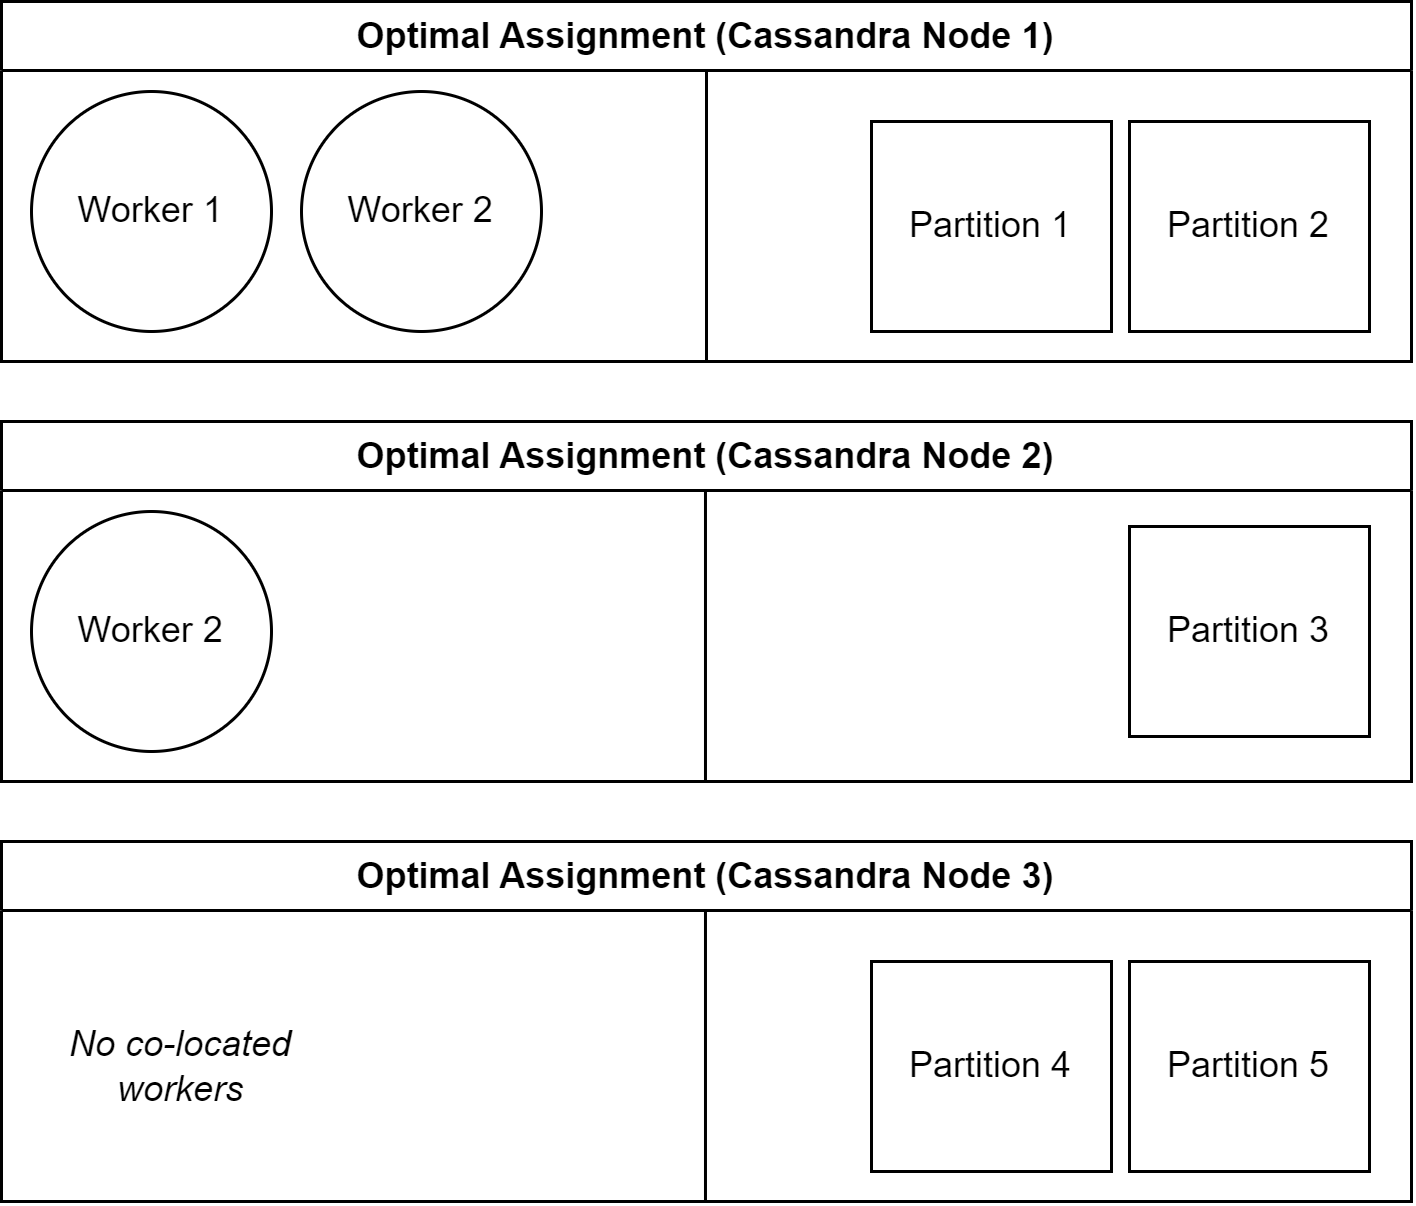
\includegraphics[width=0.8\textwidth]{chapters/diagrams/implementation/optimal-assignment-example}
	\caption{Optimal Assignment Example}
	\label{fig:optimal-assignment-example}
\end{figure}

\subsection{Group By}\label{subsec:group-by}
The Group By operation takes any number of \textit{NamedFieldExpressions} to act as unique keys, as well as any number of \textit{AggregateExpressions} which will be computed for each combination of unique keys. As with pulling source data from Cassandra, the goal when computing a Group By is for the partitions generated to be roughly equal chunks of a manageable size. To do this, two things are needed: an estimate of the full size of the dataset, and a way of splitting the dataset up to keep unique keys together. 

The process of calculating partitions and hashes, shuffling data, computing the result and deleting the original hashes is all controlled by the orchestrator during Query Plan Execution.

\paragraph{Partitions}
The first step is to compute the number of partitions that the Group By will be made up of, which is based on the size of the full dataset. To estimate this, an existing class, \textit{SizeEstimator}, was reused from Apache Spark, with some changes for compatibility with Scala 3 \cite{zaharia2016spark}. This class provides a static method \textit{estimate} which accepts any Scala object and produces an estimate, in bytes, of the size of the object. This can be called on all partial results across all workers, and the results totalled to calculate the total size of all data for a Table. Figure \ref{fig:group-by-num-partitions} shows how the size estimate can be used to derive the total number of partitions to generate for a Table.

\begin{figure}[h]
	\centering
	\[ \frac{\text{Table Size Estimate}}{\text{Goal Partition Size}} \]
	\caption{Group By - Total Partitions}
	\label{fig:group-by-num-partitions}
\end{figure}



\paragraph{Hashing} 
A unique partition is then defined as the tuple of the total number of partitions, and the partition number of this partition. Hashing, combined with the modulo operation, is used to determine which partition each row should be assigned to. In particular, Murmur3Hash is used as the hashing algorithm, which is used in Cassandra and is provided natively by Scala \cite{murmur3hash}. Figure \ref{fig:group-by-partition-assign} shows the high level equation for assigning rows to partitions. This process ensures that the new partitions will be roughly equal in size, and all rows with the same values for the unique keys will be mapped to the same partition.

\begin{figure}[h]
	\centering
	\[ Murmur3Hash(\text{Unique Key Data}) \; \%  \; \text{Total Partitions} \]
	\caption{Group By - Row Partition Assignment}
	\label{fig:group-by-partition-assign}
\end{figure} 

\paragraph{Computation}
After the hashes are computed and a worker is assigned a particular partition, it must communicate with all other workers in the cluster to get any data that relates to that partition.This ensures that the partition data is complete, and it is much the same as when the orchestrator requests query result data from the workers. The worker makes a request to all other workers, and they stream the header and rows of their partial data back to the worker that made the request. When a Group By is being computed, it's likely that a worker will be simultaneously receiving data from another worker, and sending a different set of data to it. This makes the actor system driving the data store in each worker particularly valuable, as it provides thread-safe concurrent access to the data store.

Once a worker has collected all data relating to a particular partition, it must compute the Group By result. Scala features a built-in Group By function, which this operation uses. The values for the unique keys of the Group By are calculated for each row, and the rows are placed into groups based on those values. Then, the aggregate functions are computed for each of the groups, resulting in one output row for each combination of unique keys. 

\paragraph{Deletion}
Finally, the last step of computing a Group By is to remove the hashed partition data stored on each worker, as it is no longer needed. This is handled by the orchestrator automatically during the process of computing the Group By \textit{DataSource.}

\section{Row-Level Computations}
Once partitions have been delegated to the workers, performing the computation is relatively straightforward. Included below are descriptions of how the Select and Filter operations are performed.

\subsection{Select} 
This operation takes any number of \textit{NamedFieldExpressions}. To compute a result, each \textit{NamedFieldExpression} is applied to each row of the input result. The output result has the same number of rows as the input, and fields equal to the number of \textit{NamedFieldExpressions}. 

\subsection{Filter}
This operation takes a single \textit{FieldComparison}, or a number of \textit{FieldComparisons} combined using boolean operators. To compute, each comparison is applied to each row of the input result, removing any rows where the comparison returns \texttt{false}.



\section{Query Plan}
Query plans are the process through which the orchestrator can calculate how to get from a query written by the user, to a result which it can return. A Query Plan is made up of a sequence of \textit{QueryPlanItems}, which is an interface defining one part of a query plan. Each \textit{QueryPlanItem} has an \textit{execute} method, which will make some change to the state of all workers in the cluster when called. There are four main QueryPlanItem implementations, which allow \textit{DataSources} and \textit{Tables} to be calculated and deleted.

Both \textit{DataSource} and \textit{Table} have a function that generates the full Query Plan to compute their output from scratch, as well as a second Query Plan to clean any result in the data store. 

Figure \ref{fig:filter-group-by-query-plan} shows the query plans for the Filter and Select query (\ref{fig:filter-select-query}) and Group By Query (\ref{fig:group-by-query}).

\begin{figure}
	\centering
	\subfloat[\centering Filter and Select Query]{{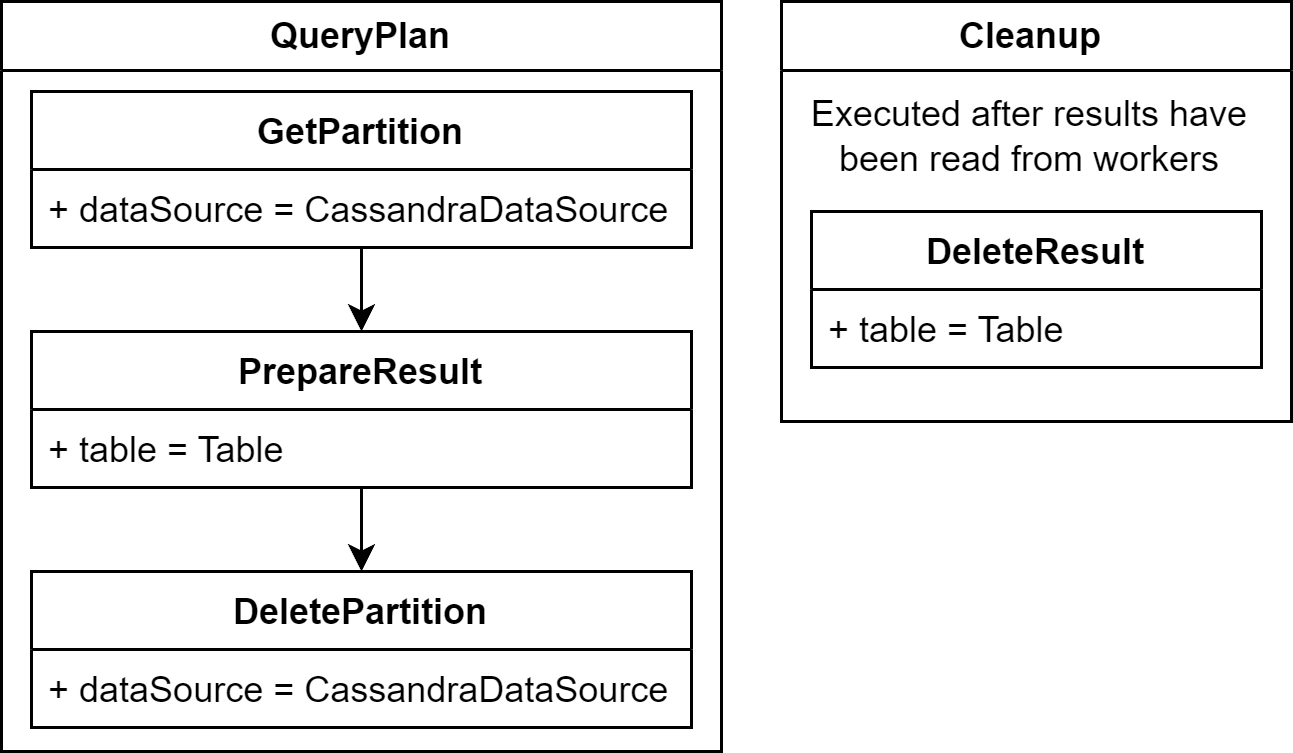
\includegraphics[width=0.3\textwidth]{chapters/diagrams/implementation/filter-select-query-plan}}}
	\qquad
	\subfloat[\centering Group By Query]{{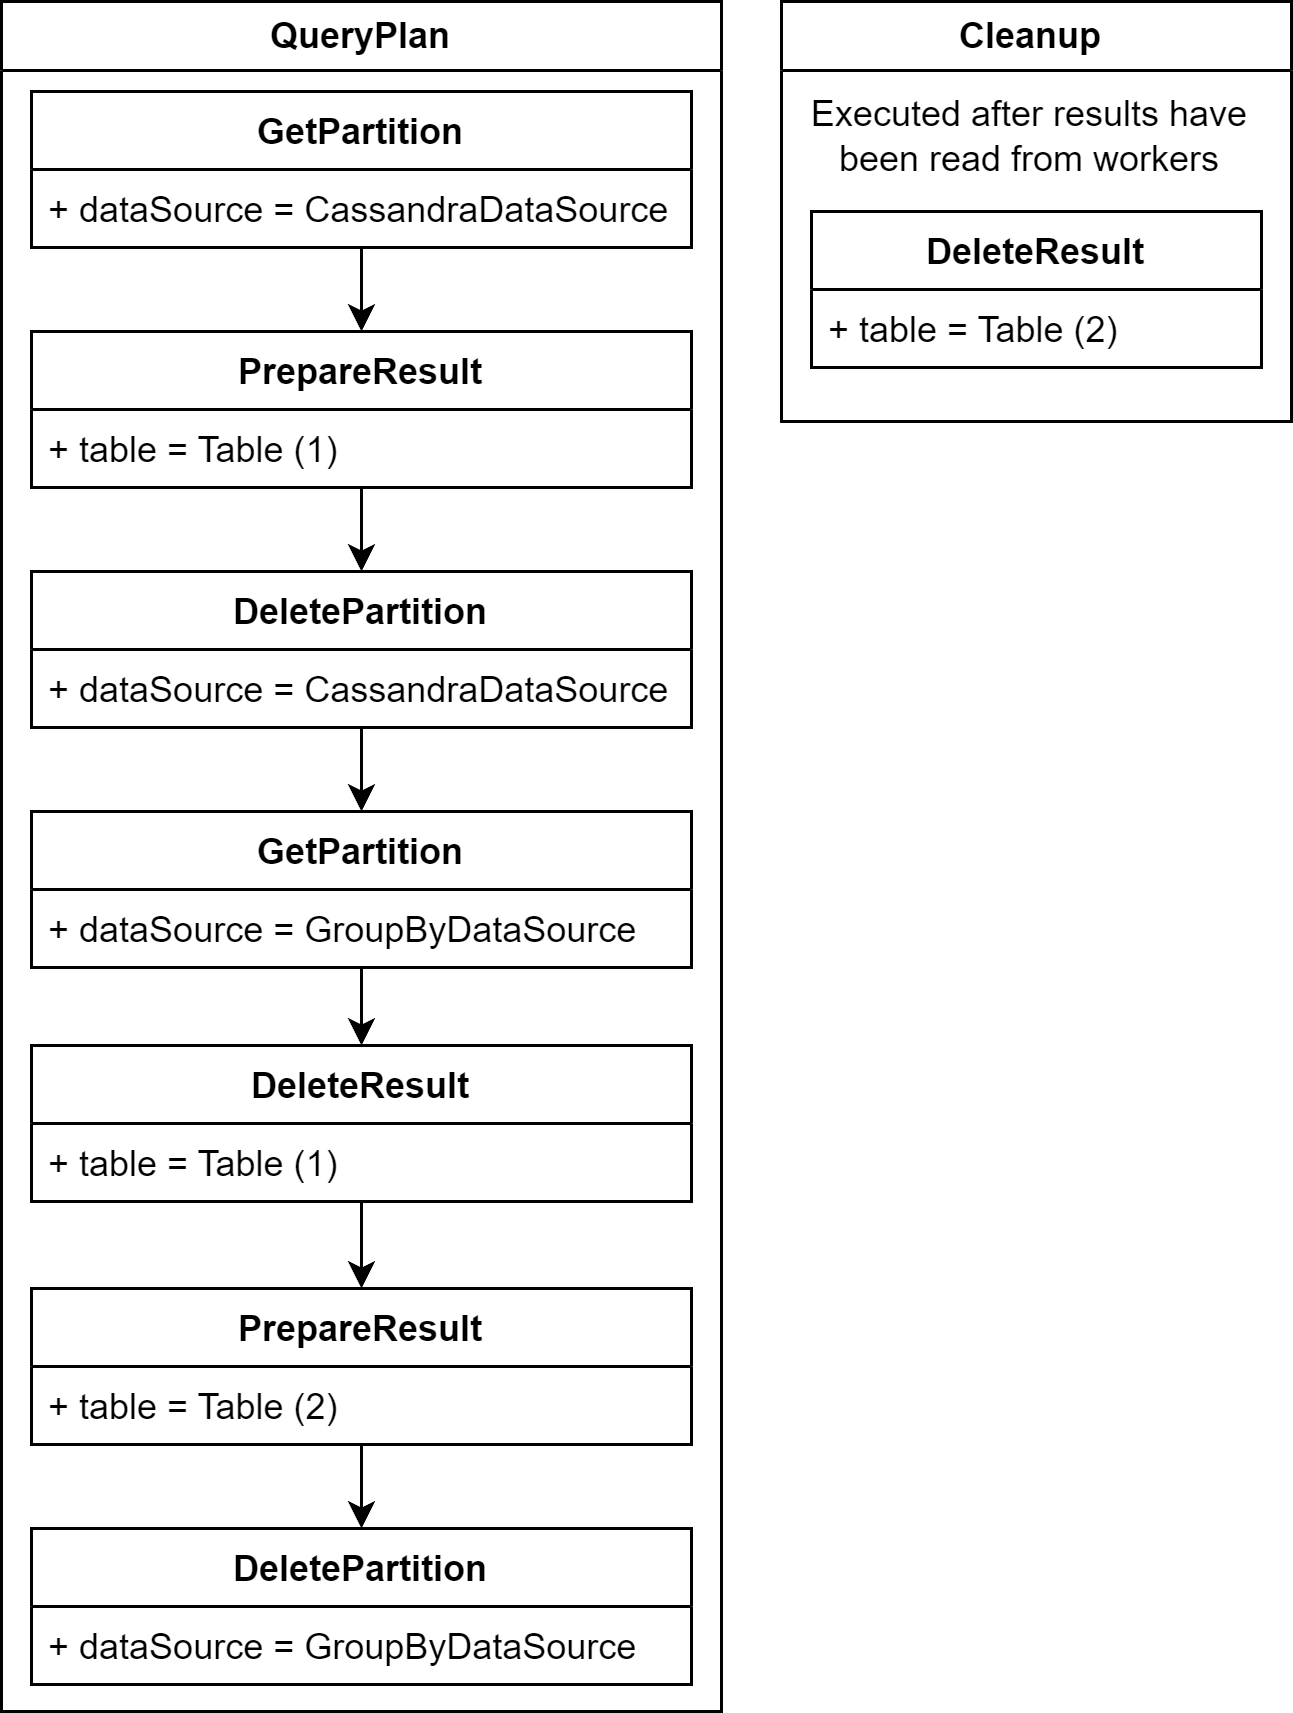
\includegraphics[width=0.3\textwidth]{chapters/diagrams/implementation/group-by-query-plan}}}
	\caption{Query Plans - Filter-Select and Group By Query}%
	\label{fig:filter-group-by-query-plan}
\end{figure}

\subsection{GetPartition}
This is the most complex \textit{QueryPlanItem}, encapsulating a number of steps in order to compute and store the partitions of a \textit{DataSource}. There are two main flows depending on if the \textit{DataSource} has dependent Tables.

If the \textit{DataSource} has no dependencies, for example when pulling data from Cassandra, then Figure \ref{fig:get-partition-no-dependencies} shows the process for this item. 

\begin{figure}[h]
	\centering
	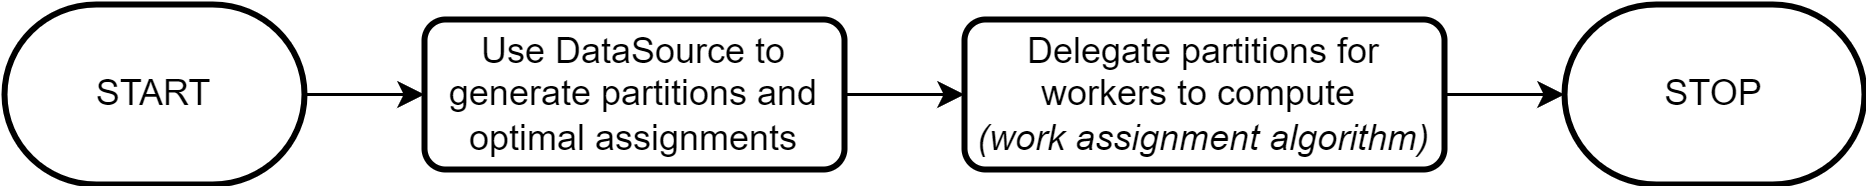
\includegraphics[width=0.8\textwidth]{chapters/diagrams/implementation/get-partition-no-dependencies-flow}
	\caption{Get Partition Execution - Without Dependencies}
	\label{fig:get-partition-no-dependencies}
\end{figure}

If the \textit{DataSource} has dependencies, then Figure \ref{fig:get-partition-dependencies} shows the process for this item. First, the partitions and optimal assignments are generated, then the dependency data is hashed based on the number of partitions to generate. Both of these steps are implementation-specific, and are therefore abstracted behind the \textit{DataSource} interface. The work assignment algorithm is then run to delegate partitions to the workers, followed by deleting the hashed dependency data. These steps do not change based on the \textit{DataSource}, so are handled exclusively by \textit{GetPartition}. These steps are the same as when calculating a Group By (Section \ref{subsec:group-by}), which is an implementation of \textit{DataSource}.

\begin{figure}[h]
	\centering
	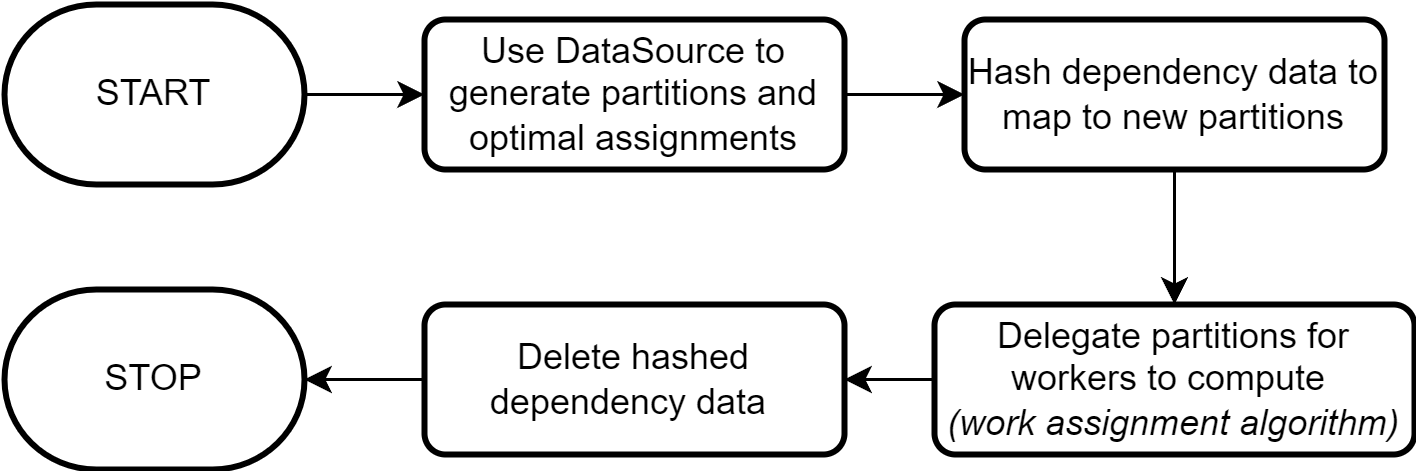
\includegraphics[width=0.7\textwidth]{chapters/diagrams/implementation/get-partition-dependencies-flow}
	\caption{Get Partition Execution - With Dependencies}
	\label{fig:get-partition-dependencies}
\end{figure}

\paragraph{Work Assignment Algorithm}
The details of how the partitions are actually computed are abstracted behind the \textit{DataSource} interface as they are implementation specific, but GetPartition always needs to manage the process of sending requests to the workers to compute the partitions. This is done using the Work Assignment Algorithm. 

A simple solution would be to use a round-robin process to match optimal assignments to their workers, delegating work when a request finishes and stopping when the assignment list is empty. However, this can result in idle workers, for example if one worker's list of optimal assignments is shorter than the others, or if one worker takes unexpectedly long to complete their work.

The ideal solution would ensure a worker computes all of its own optimal partitions first and, once these are complete, computes the partitions that were originally assigned to other workers. This implements a form of dynamic load balancing, because a faster-running worker is able to take on more requests than a slower worker, and no worker will be idle unless there are no partitions left to compute. However, this presents concurrency challenges, including preventing race conditions like the same partition being delegated twice to different workers.

The actor model, used previously in the data store, is ideal for this situation. Sets of optimal partitions are modelled as \textit{producer} actors, and the workers as \textit{consumers}. Producers respond to requests for work with partitions to be computed. Consumers are provided with an ordered list of producers, then repeatedly request and compute work from each in order. Each consumer is given a differently ordered list, with the producer of that consumer's optimal partitions placed first in the list. When all assigned producers for a consumer are empty, the consumer will shut down. The final part of the system is a counter, which tracks the number of completed partitions, sending a signal when all partitions have been computed, or an error if any worker fails.

This solution also handles the case where no worker is co-located with a set of partitions; this producer will simply be placed last in the list of producers for each consumer, resulting in these partitions eventually being processed.

Figure \ref{fig:producer-consumer-model-example} provides the initial state of this model, using the example optimal assignment in Figure \ref{fig:optimal-assignment-example}. Dark arrows represent the producer which the consumer will empty first, containing its optimal assignments. Light grey arrows represent the other producers which the consumer can access. Note that Producer 3 is not the first producer for any worker, but will eventually be checked by the workers when all other producers are exhausted.

\begin{figure}[h]
	\centering
	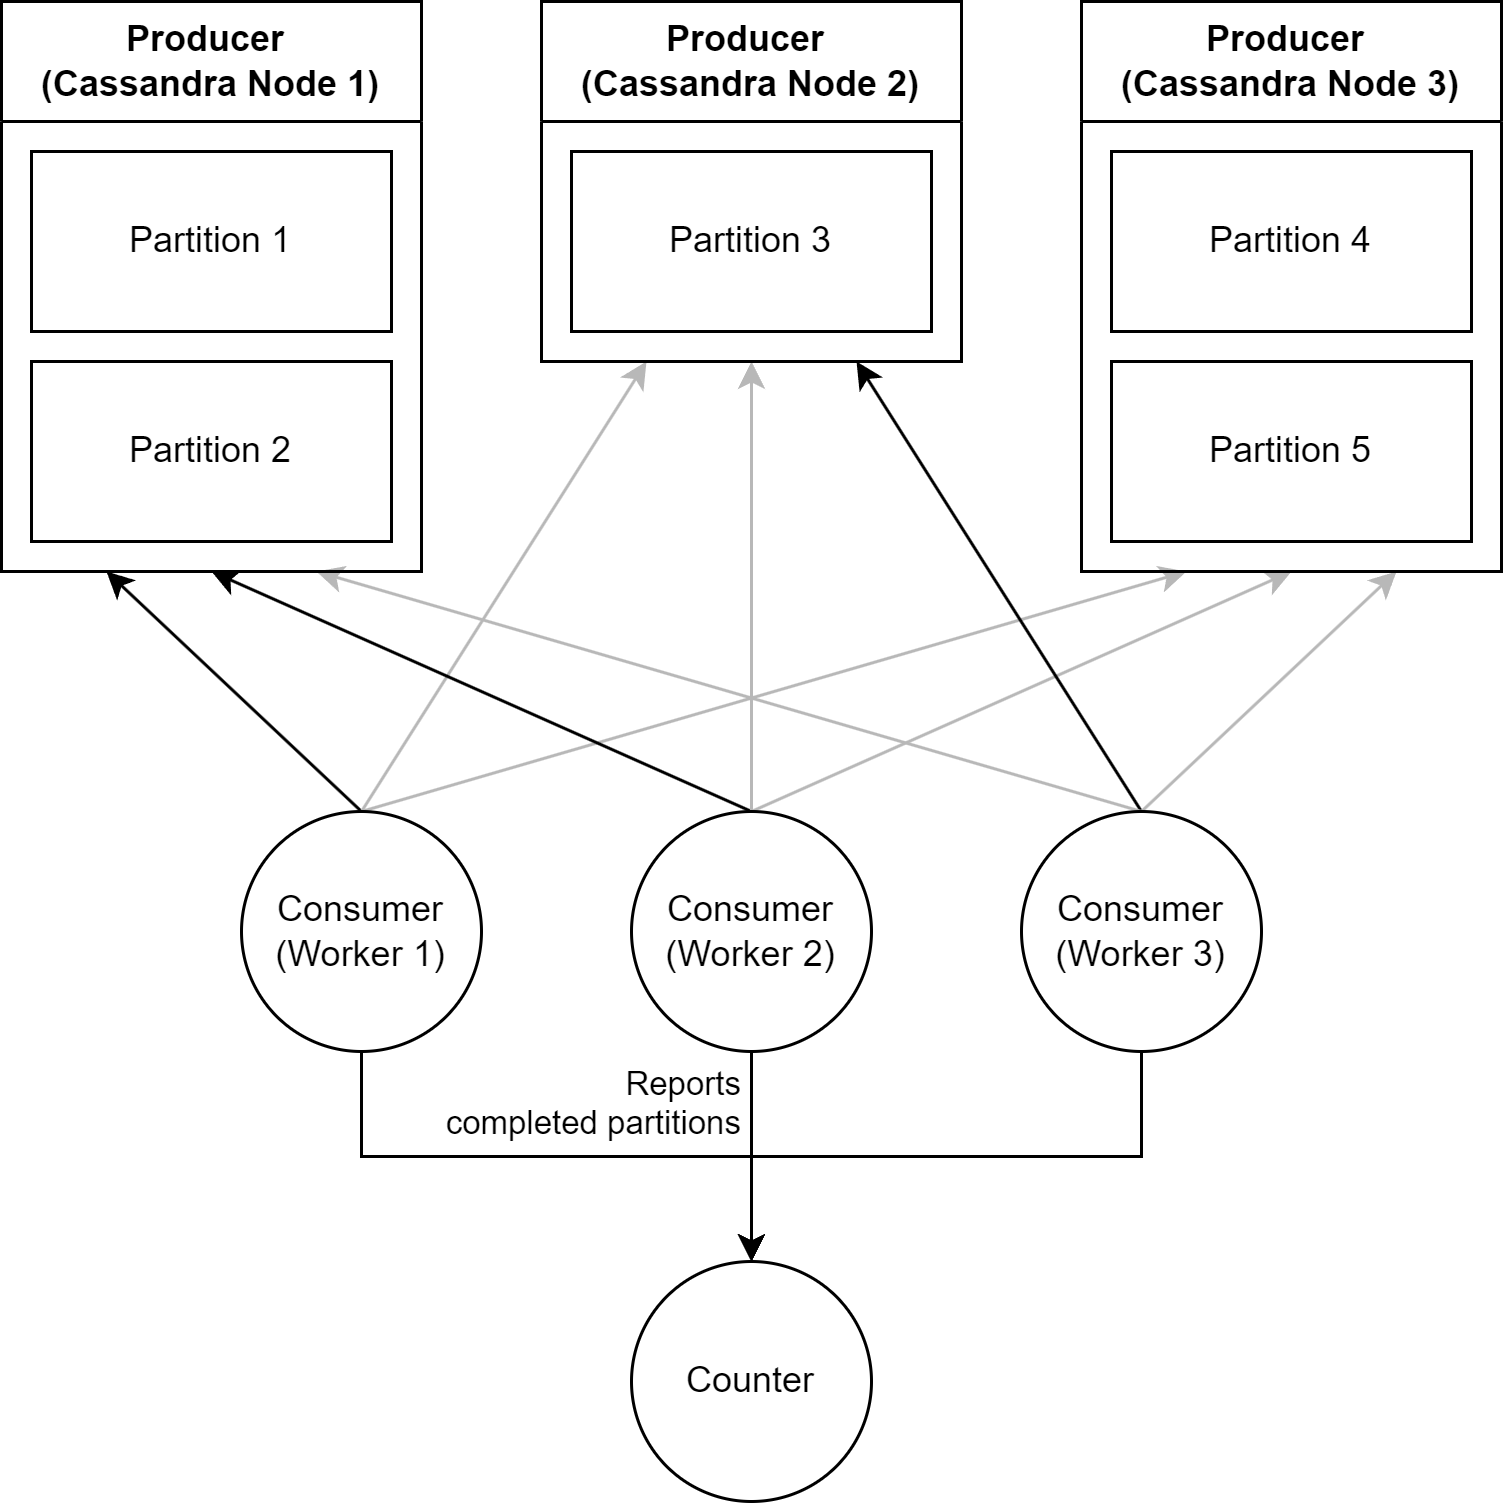
\includegraphics[width=0.5\textwidth]{chapters/diagrams/implementation/producer-consumer-model-example}
	\caption{Producer Consumer Model Example}
	\label{fig:producer-consumer-model-example}
\end{figure}

\subsection{PrepareResult}
This \textit{QueryPlanItem} computes a Table from the partitions of a \textit{DataSource} that are already stored on the workers. Therefore, it will always be called after GetPartition, with the partitions generated by \textit{GetPartition} as an argument. The implementation uses a modified version of \textit{GetPartition}'s actor system, which iterates through all partitions on each worker, sending a request for each partition to perform the \textit{Table} computation.

\subsection{DeleteResult and DeletePartition}

\textit{DeletePartition} and \textit{DeleteResult} are \textit{QueryPlanItems} for removing the results of a \textit{GetPartition} and \textit{PrepareResult} operation, respectively. These will send a single request to each worker, and they will remove all results that relate to a \textit{Table} or \textit{DataSource}, and respond with a confirmation.

\subsection{Result Collation}
After all the steps of a query are completed, the final results are stored across all the workers. The orchestrator makes a request to all workers to return the computed results, and each worker iterates over all partial results in the data store, streaming the data back to the orchestrator. An actor system is used to pipe the concurrent responses from all workers into a single thread, which combines the results and streams them to the frontend. 

The request is initiated by the orchestrator, rather than the workers pushing data to the orchestrator, because gRPC requires that one system act as a server, and another as a client. For the query plan model, it makes most sense for the workers to be servers, so this much also be the case for result collation.

\section{Deployment}
As discussed in Chapter \ref{cha:design}, Kubernetes was chosen to manage all nodes in the cluster. One of the key features that makes it useful for the system are scheduling rules, which provide Kubernetes with information about how containers should be assigned to physical nodes.

As previously described in \ref{subsec:colocation}, worker nodes will determine their closest Cassandra node automatically based on latency. To make the best use of the cluster, workers should be distributed evenly across all nodes that have a Cassandra node, and the following two scheduling rules will provide this:
\begin{enumerate}
	\item Workers should be placed on the same Kubernetes node as a Cassandra node if possible.
	\item Workers should not be placed on the same node as other worker nodes.
\end{enumerate}

The scheduling rules are expressed as preferences rather than requirements, Kubernetes is still able to schedule the nodes if there are more workers than Cassandra nodes.

\subsection{CI/CD}
To aid in deploying to Kubernetes, continuous integration/continuous deployment (CI/CD) pipelines are used for each of the components of the system, specifically using GitHub Actions \cite{githubactions}. Each pipeline runs all unit tests for the component, and provided they succeed, builds a docker container and pushes it to a container registry, ready for use in the Kubernetes cluster.


	
	\chapter{Testing}\label{cha:testing}

% Covers unit tests, and performance tests

As discussed in Chapter \ref{cha:intro}, the high level aim of this system is to improve the speed of data processing for large datasets. Therefore, it is important to conduct performance testing of the overall system. This section aims to cover a number of methods in which the performance of the completed solution is evaluated.

Firstly, raw performance testing is conducted against a typical data processing solution, Microsoft SQL Server. Then, a number of alternative approaches are assessed for determining how well the cluster leverages the parallelisation of running the computation over multiple nodes.

\section{Unit Tests}
Thorough unit testing is important for any software engineering focused project. By writing tests throughout development, the expected behaviour of individual components in the system can be validated. Through the use of continuous integration/continuous deployment (CI/CD) pipelines, this behaviour can continue to be validated as other parts of the system are improved, to ensure changes do not break the behaviour of the component. 

Scalatest was chosen as the unit test framework \cite{scalatestuserguide}. Furthermore, both gRPC and Akka Actors provide classes for writing unit tests around the frameworks, and this is combined with Mockito to mock any dependencies that cannot be run during testing like the Cassandra Driver \cite{scalatestplusmockito, datastaxjavadriver}. Using these tools and frameworks, unit tests have been written for the majority of core code; this includes the DSL, query model and partitioning code among other classes. In total, more than 350 individual tests were written for this project, split across the Python frontend, core code, orchestrator and worker code.

\section{Test Data}
To aid performance testing, fake data is created to test the different operations of the system, produced based on discussions with potential users of the system. The intended users have a financial background, as they work within Audit at PwC, so the chosen test data is loan origination (creation) data. A short Python script generates this data by randomising a number of fields between specified bounds. Figure \ref{fig:fake-loan-data} shows ten example records of the data.

\begin{figure}[ht]
	\centering
	\begin{tabular}{| l | l | l | l | l |}
		\hline
		\textbf{Loan ID} & \textbf{Amount} & \textbf{Interest Rate} & \textbf{Duration (Yrs)} & \textbf{Origination Date} \\ \hline 
		0 & 590,418 & 0.041139 & 24 & 2021-04-23 18:13:00   \\ \hline
		1 & 697,824 & 0.095023 & 20 & 2021-10-06 20:07:00    \\ \hline
		2 & 271,853 & 0.029358 & 23 & 2021-03-08 05:12:00    \\ \hline
		3 & 329,950 & 0.038111 & 23 & 2021-01-18 21:05:00    \\ \hline
		4 & 1,381,994 & 0.055411 & 30 & 2021-05-13 15:54:00  \\ \hline
		5 & 1,365,793 & 0.0093872 & 29 & 2021-05-04 03:18:00  \\ \hline
		6 & 1,143,926 & 0.078929 & 21 & 2021-07-11 19:10:00   \\ \hline
		7 & 461,215 & 0.082520 & 23 & 2021-05-04 17:50:00    \\ \hline
		8 & 287,307 & 0.040382 & 21 & 2021-05-20 06:08:00   \\ \hline
		9 & 191,668 & 0.061314 & 25 & 2021-09-03 16:21:00    \\ \hline
	\end{tabular}
	\caption{Example Loan Origination Data}
	\label{fig:fake-loan-data}
\end{figure}

\section{SQL vs Cluster Solution}
This section will compare the performance of an instance of Microsoft SQL Server, against the completed solution, referred to as the Cluster Processor in this testing. 

\paragraph{Test Plan}
The tests are conducted for the three types of query that the cluster processor supports: Select, Filter and Group By. Within each type of query, a simple, and a complex version of the query will be written and tested. For the cluster processor, the tests are run tables containing loan origination data with the following number of rows: 1000, 10000, 100,000, 1 million and 10 million rows. For SQL, tables with the same number of rows are generated, as well as two further tables: 50 and 100 million rows. These are included to provide further context of how SQL scales at larger data volumes; the cluster processor was unable to test these tables due to time and cost constraints.

To reduce the effect of random error, each test is run 5 times, and the results averaged across all tests. This is particularly important when running on a cloud environment, as there is less control over the hardware running the tests. In particular, there is no control over what other work that hardware is doing alongside the testing, so averaging a number of results should reduce any impact this has.

In all of these tests, Microsoft SQL Server was running on an instance of Azure SQL Database \cite{azuresqldatabase}. The Cluster Processor was running on Azure Kubernetes Service, with a pool of three nodes available, each node having 4 vCores, and 16GB memory \cite{azurekubernetesservice}. The actual CPU and memory available to each pod in the cluster is controlled by Kubernetes.

\subsection{Controls}
A number of variables must be considered which could have an impact on the results of this test. The testing attempts to mitigate the effects of these variables in order to make the results as comparable as possible.

\paragraph{CPU and Memory}
At larger data volumes, CPU and Memory is the biggest contributing factor that will affect how quickly the computation is performed, both on SQL and the Cluster Processor. Ensuring these are comparable is essential for producing reliable test results. For Azure SQL Database, a slider can be used to set the maximum number of vCores available, and a set amount of memory is assigned based on the number of cores. In this case, a maximum of 6 vCores were used, which results in of 18GB memory accessible to the database.

As the Cluster Processor is running on Kubernetes, granular control over the number of vCores and amount of memory available to each node is possible using resource limits \cite{k8sapi}. Workers were configured to have a maximum of 2 vCores, and 6GB memory available to each, with 3 workers in total. As a result, the cluster as a whole has 6 vCores and 18GB memory available, the same as the SQL database.

\paragraph{Network Latency}
Controlling network latency is particularly important for small data volumes which resolve quickly. For a request that takes 0.5s to complete, 100ms of latency will make the completion 20\% slower. Testing was always performed on an instance of Azure Cloud Shell, which is a terminal running inside the same Azure datacenter as the test environment \cite{azurecloudshell}. This ensures the network latency is minimised and comparable between environments, with 16ms average round-trip time for a TCP ping to both SQL server, and the Cluster Processor.

\paragraph{Warm-Up}
Both SQL and Cluster Processor have a warm-up periods when they are first started. Azure SQL Database is run using a serverless computation style, which means the server is scaled to 0 resources when it is unused. This has the disadvantage that when a query is first run, there is a short delay while the resources are provisioned again. Cluster Processor has a similar warm-up when it is first started, because the gRPC connections between the orchestrator and workers are not actually created until the first request is made. To overcome both of these warm-up periods, a number of queries are run just before testing begins, and the time taken to run these is not tracked.

\subsection{Select Query}
The first query is a pure select, which essentially tests how fast both solutions can send results over the network. Figure \ref{fig:sql-select-simple} shows the SQL query, and Figure \ref{fig:cluster-select-simple} shows the Cluster Processor query. The second select query is a more complex select, with some conversion operations to test if this has an impact on the computation time. Figures \ref{fig:sql-select-complex} and \ref{fig:cluster-select-complex} show the queries.

\paragraph{Results} The results for this query are shown in Figure \ref{fig:select-graph}. Data is only available for Cluster Processor up to 100,000 rows because of a memory issue when passing data from the workers to the orchestrator, which is analysed further in Chapter \ref{cha:evaluation}. As a result, the graph is filtered to exclude the SQL results for 50 and 100 million rows.

However, the data that is available shows that the Cluster Processor is more than 10x slower at performing Select queries than SQL. This is most likely related to the format used to send the result data, which requires serialising both the type and value of each cell in the data for transmission. For both SQL and the Cluster Processor, there is no significant difference between the raw Select, and the Select with operations. The largest difference is at 100k rows for Cluster Processor, where there is a 0.3s increase when computing the operations compared to a raw Select.

\begin{figure}[htp]
	\centering
	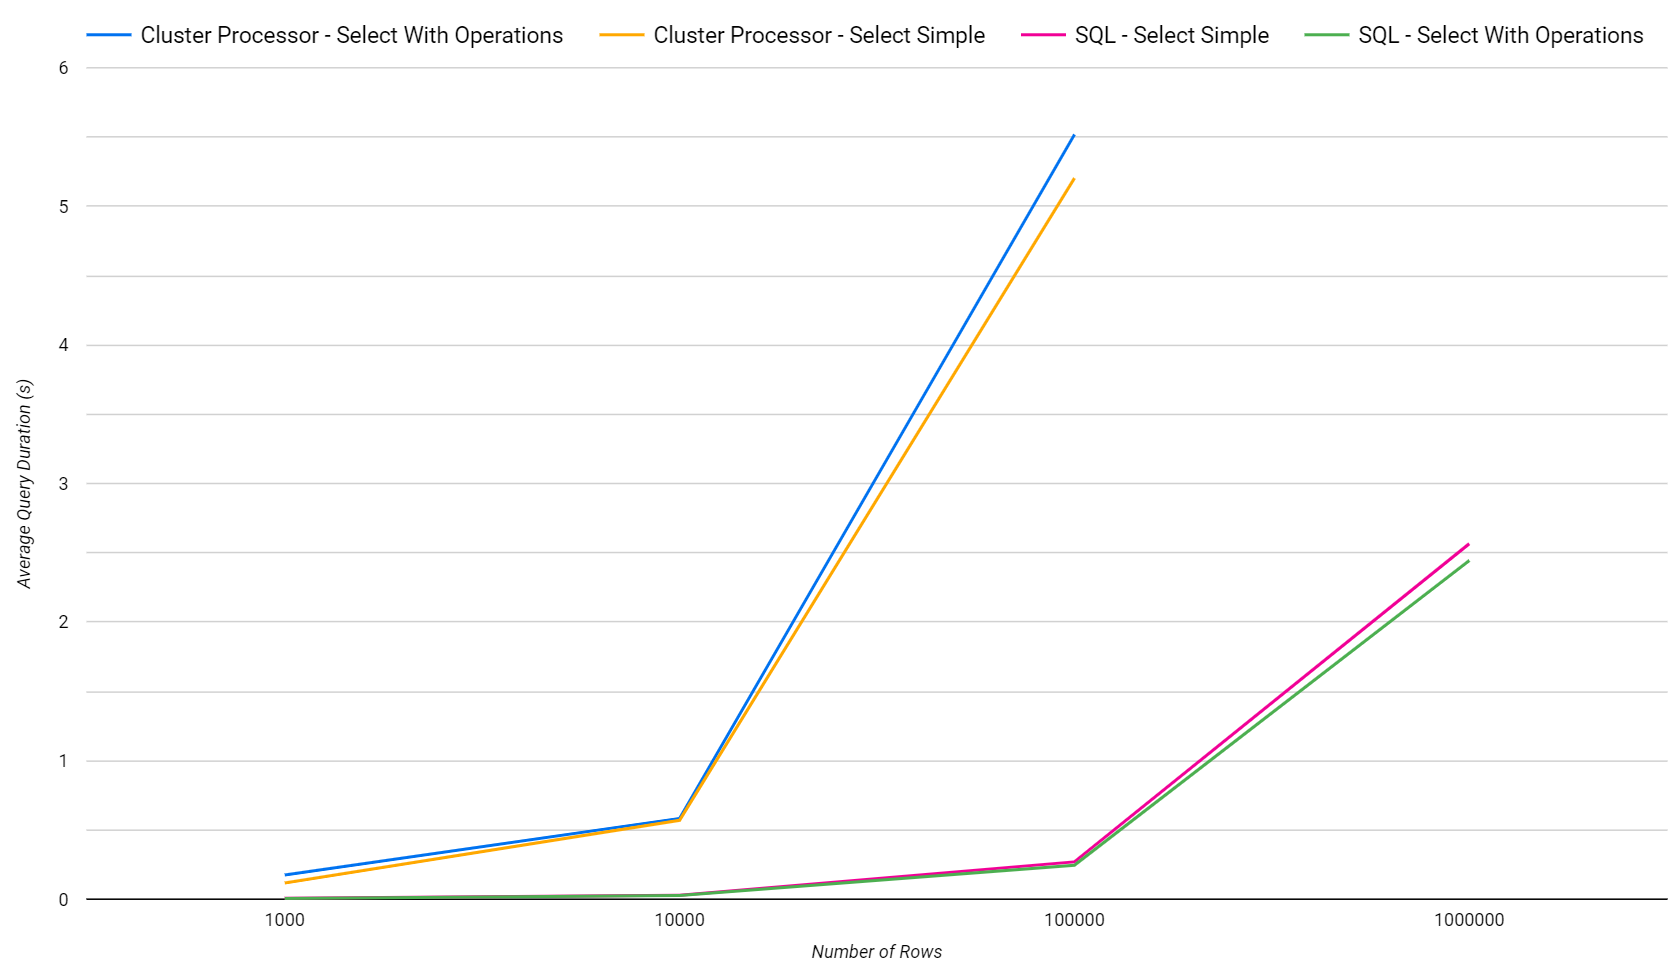
\includegraphics[width=0.8\linewidth]{chapters/diagrams/testing/select-simple-1k-1m}
	\caption{SQL vs Cluster Processor - Select Query Results}
	\label{fig:select-graph}
\end{figure}

\subsection{Filter Query}
The first query is a simple filter, with no AND/OR combinations. Figures \ref{fig:sql-filter-simple} and \ref{fig:cluster-filter-simple} show the queries. The second filter is more complex, testing both boolean operators. Figures \ref{fig:sql-filter-complex} and \ref{fig:cluster-filter-complex} show the queries.
The results for this query are shown in Figure \ref{fig:filter-graph}. 

\paragraph{Results}
The results for this query are shown in Figure \ref{fig:filter-graph}, where testing was performed for the full range of datasets in both SQL and the Cluster Processor. The results show that SQL is again significantly faster in this test case, producing results around 15-20x faster. This is likely to be partially caused by the transmission format, as with the Select queries. However, it is also likely that SQL is able to exploit caching more extensively over repeated tests when compared to the Cluster Processor, particularly with the smaller tables which can be held in memory permanently. This is because the Cluster Processor fetches fresh data from Cassandra every time the query is called.

Another relevant insight from this data is that the complex filter reliably executes faster than the simple filter across all results. For the Cluster Processor, it is nearly 2 seconds faster on average at 10 million rows, and for SQL it is almost 6 seconds faster at 100 million rows. This is to be expected, since the complex filter is  more restrictive in the results that it returns, so there is less data to transfer over the network.

\begin{figure}[htp]
	\centering
	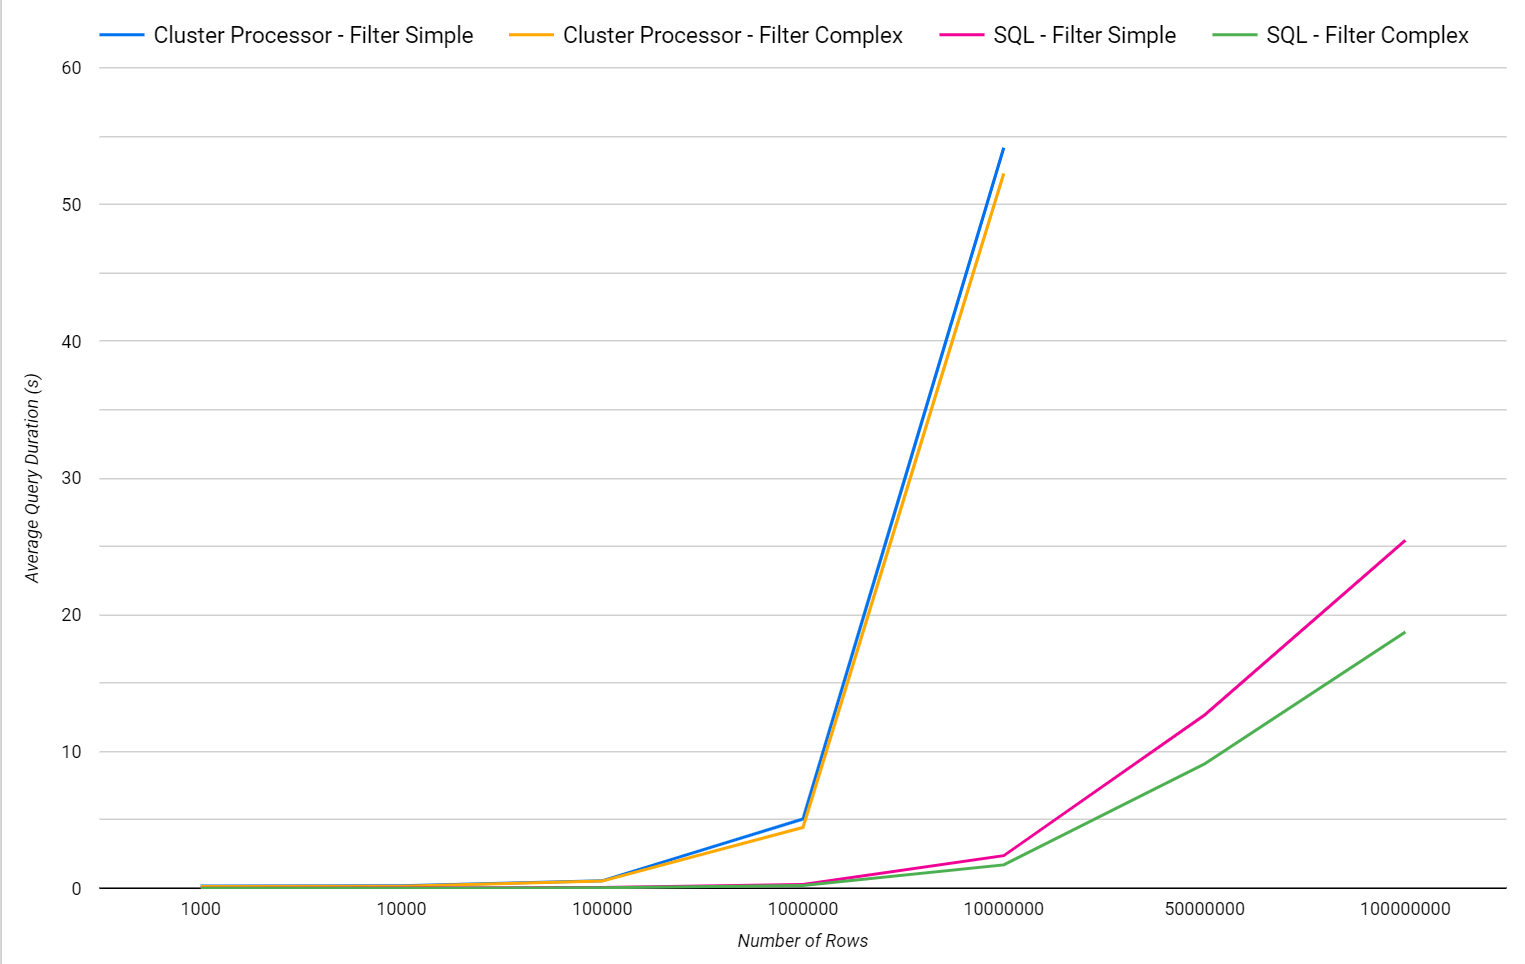
\includegraphics[width=0.8\linewidth]{chapters/diagrams/testing/filter-1k-100m}
	\caption{SQL vs Cluster Processor - Filter Query Results} 
	\label{fig:filter-graph}
\end{figure}


\subsection{Group By Query}
The first query is a simple group by, essentially acting as a \texttt{DISTINCT} check. Figures \ref{fig:sql-group-by-simple} and \ref{fig:cluster-group-by-simple} show the queries. The second group by is more complex, featuring a number of aggregations. Figures \ref{fig:sql-group-by-complex} and \ref{fig:cluster-group-by-complex} show the queries. 

\paragraph{Results}
The results for this query are shown in Figure \ref{fig:group-by-graph}, where again testing was performed for the full range of datasets in both solutions. SQL is significantly faster, and scales much better as the data sizes increase. For the Cluster Processor, the aggregate group by is over twice as fast on average than the simple version at 10 million records. The testing was performed sequentially, with no break between tests, so it is unclear why this result is so much faster. Furthermore, the same difference in computation time is not present at smaller data volumes. This could be caused by the less controlled cloud environment, meaning perhaps some unexpected load was present during the simple test which resulted in slower computation. Another round of testing would need to be performed to determine if this was the case.

Despite this unexpected difference in computation times between the queries at 10 million rows, there is still a significant performance drop-off when compared to the results at 1 million records. Analysing the outputs from the workers at this data volume, the results could not be stored entirely in-memory, resulting in a large amount of computation time being spent swapping partial results to and from disk. Group By operations suffer from memory shortages worse than other types of queries, as around twice the normal data volume is stored at one time; the source data for the Group By, data for the new hashes, and the newly computed group by partitions are all kept in the data store at the same time.

\begin{figure}[htp]
	\centering
	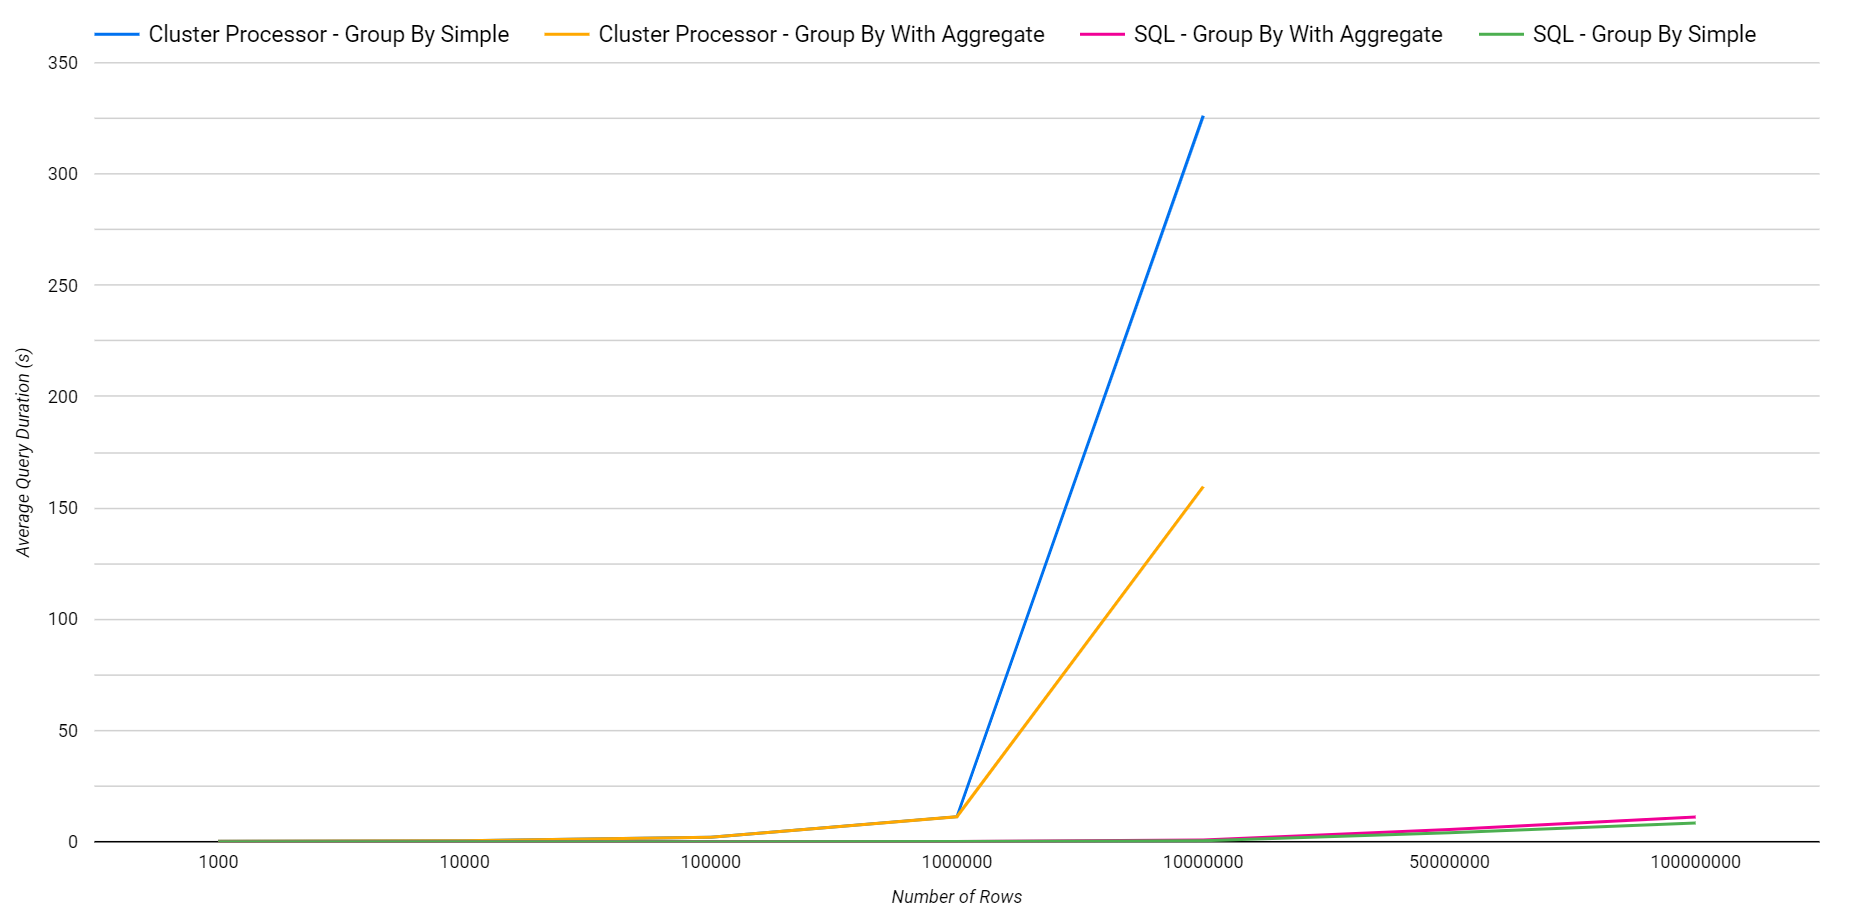
\includegraphics[width=0.8\linewidth]{chapters/diagrams/testing/group-by-1k-100m}
	\caption{SQL vs Cluster Processor - Group By Query Results}
	\label{fig:group-by-graph}
\end{figure}

\subsection{Analysis}
As the raw performance testing results show, a significant amount of optimisation would be required for the Cluster Processor solution to truly compete with SQL with regards to computation speed. In particular, the system appears to be weakest at transmitting raw data quickly across the network, as well as computing Group Bys quickly.

One way the transmission format for results could be optimised is to reduce the size of the serialised row data. Currently, every value within a row also stores type information, but this information has already been sent as part of the header. Therefore, the system could stop sending type information with the value data, then use the header to perform a conversion when the row is received. 

% What's the impact of the calculations, and what's the impact of the network on the results?
The main inefficiency that causes the poor Group By performance is the workers holding onto more data than necessary. Currently for simplicity, the workers hash a copy of all rows in the data before cross-communication occurs. It should be possible to partially perform the Group By operation for each partition on each worker, then finalise those partial results on the worker that actually holds the partition, significantly reducing the amount of stored and transferred data. As testing has already established that the raw data transmission is suboptimal, by sending more data than is required, the network inefficiencies have a larger impact on performance. Furthermore, when computing Group Bys at 1 million rows, the workers ran low on free memory, and began spilling data to disk. This is significantly slower than only in-memory storage, so by reducing the amount of stored data, spilling would occur at larger data volumes, and performance would be improved.

\section{Level of Parallelisation}\label{sec:parallelisation-test}
This section will compare the performance of the Cluster Processor when the number of workers is varied, but the overall performance in terms of available resources is the same. The aim is to determine how changing the level of parallelisation in the cluster impacts the computation speed. 

In these tests the simple versions of the Select, Filter and Group By queries were executed, with a different range of rows depending on the test. See Appendix \ref{cha:testing-figs} for details of the queries that were executed. Figure \ref{fig:parallelisation-test-workers} shows the cluster layouts for each test case; the number of workers, and the resources available to each worker. As shown, the overall number of vCores and GB of memory available to the cluster is the same in each case.

Throughout all of these tests, the number of Cassandra nodes in the cluster remained consistent: 3 nodes, one placed on each Kubernetes node.

\begin{figure}[ht]
	\centering
	\begin{tabular}{| c | c | c | c | c |}
		\hline
		\textbf{Workers} & \textbf{vCores} & \textbf{Worker Memory} & \textbf{Total vCores} & \textbf{Total Memory} \\ \hline
		2 & 3 & 9GB & 6 & 18GB \\ \hline
		3 & 2 & 6GB & 6 & 18GB \\ \hline
		6 & 1 & 3GB & 6 & 18GB \\ \hline
		9 & 0.666 & 2GB & 6 & 18GB \\ \hline
		12 & 0.5 & 1.5GB & 6 & 18GB \\ \hline
	\end{tabular}
	\caption{Parallelisation - Number of Workers and Resources}
	\label{fig:parallelisation-test-workers}
\end{figure}

\subsection{Select Query}
The results of this test are shown in Figure \ref{fig:select-simple-parallelisation-test}. Due to the same memory issue as in the SQL test, only 1000 to 100000 row tables were tested. The cluster layout with 3 nodes appears to execute around twice as fast across all data volumes compared to the other layouts, which all have similar execution times on average. Ultimately, this test is checking how fast each layout can pull data from Cassandra, and send it to the Orchestrator. It is likely that the extra overhead introduced by the higher levels of parallelisation slowed down data transfer, and there was no computation to perform which would benefit the increased number of nodes. 

However, at 100,000 rows the 9 node cluster ran marginally faster than the other slow layouts. These are still tightly clustered with all results within 0.4s of one another, suggesting this is likely caused by random variation, rather than the 9 node cluster being specifically faster. Further testing, particularly at higher data volumes, would be required to confirm any trends here. 

Interestingly, the 2 node cluster also performed slower than the 3 node cluster. This is likely because this layout has one less worker node than Cassandra node, meaning latency is added to retrieve data from the Cassandra node without a co-located worker. 

\begin{figure}[ht]
	\centering
	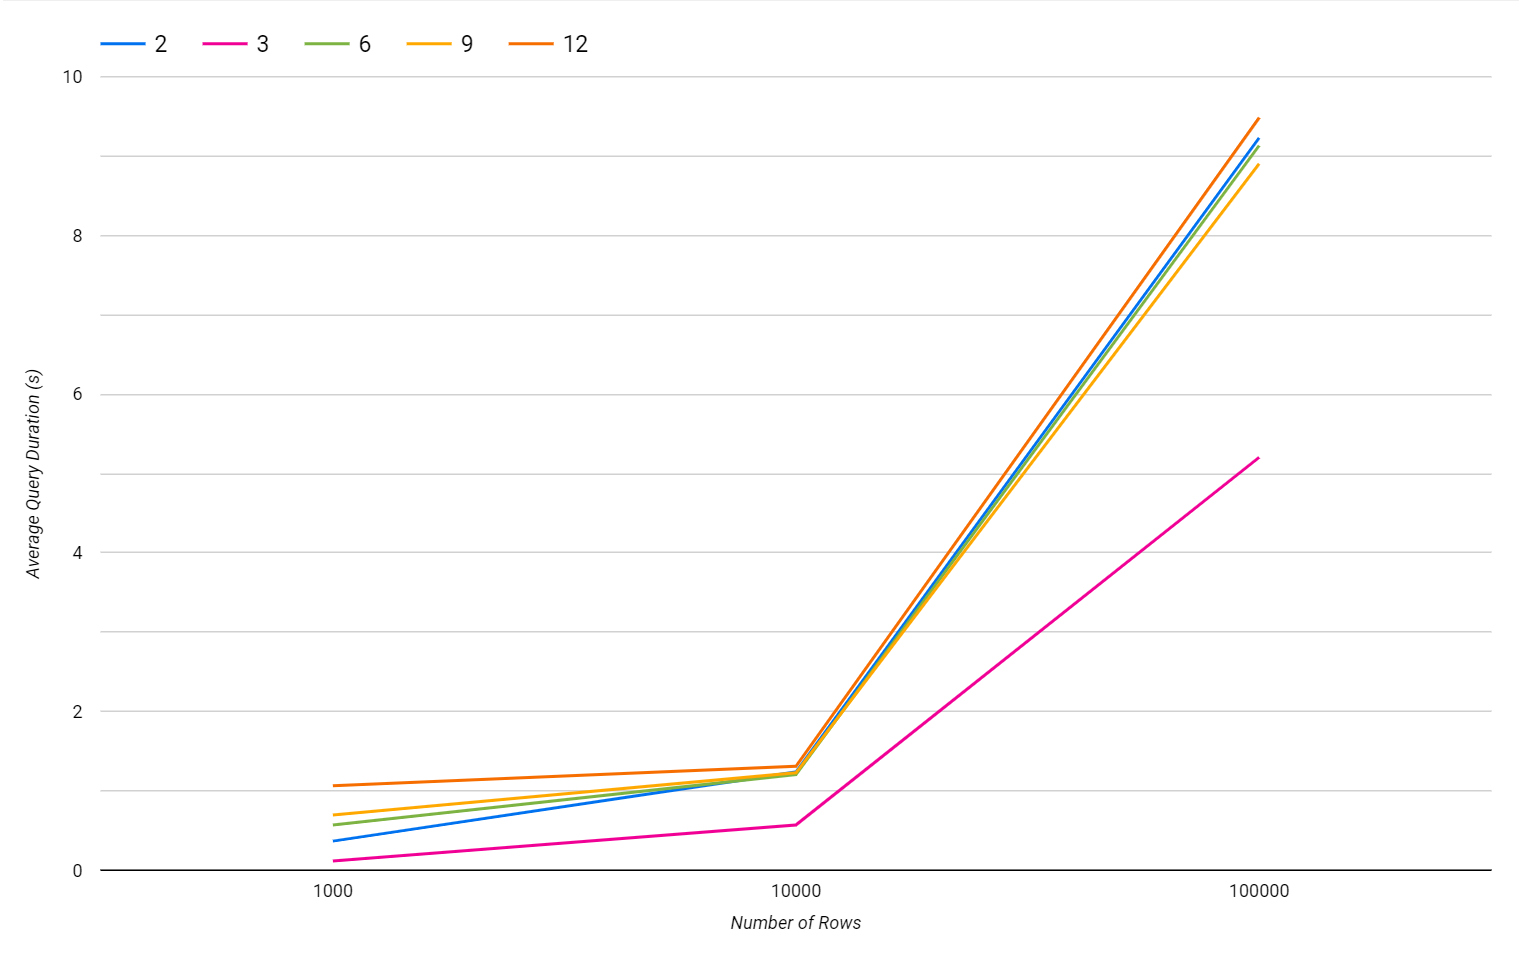
\includegraphics[width=0.8\linewidth]{chapters/diagrams/testing/select-simple-parallelisation-test}
	\caption{Parallelisation - Select Query Results} 
	\label{fig:select-simple-parallelisation-test}
\end{figure}

\subsection{Filter Query}
The results of this test are shown in Figure \ref{fig:filter-simple-parallelisation-test}. At small numbers of rows, there is very little difference between each of the cluster layouts. However, an interesting trend appears as the number of rows increases above 100,000. The 3 node cluster is fastest until this point, but is then overtaken by the 9 node cluster at 1 million.

To investigate this trend further, the test was also run for all cluster layouts at 10 million rows, shown in Figure \ref{fig:filter-simple-parallelisation-10m}. At this number of rows, the layouts with 6, 9 and 12 nodes are all faster than the 3 node cluster, with 9 nodes appearing to be the optimal level of parallelisation. This shows that as the amount of work increases, the increased level of parallelisation becomes a benefit, resulting in faster computation times. The fact that 12 nodes is slower than 9 nodes at 10 million rows suggests that there is an optimal point in terms of maximising parallelisation, without introducing too much overhead from the number of nodes.

\begin{figure}[ht]
	\centering
	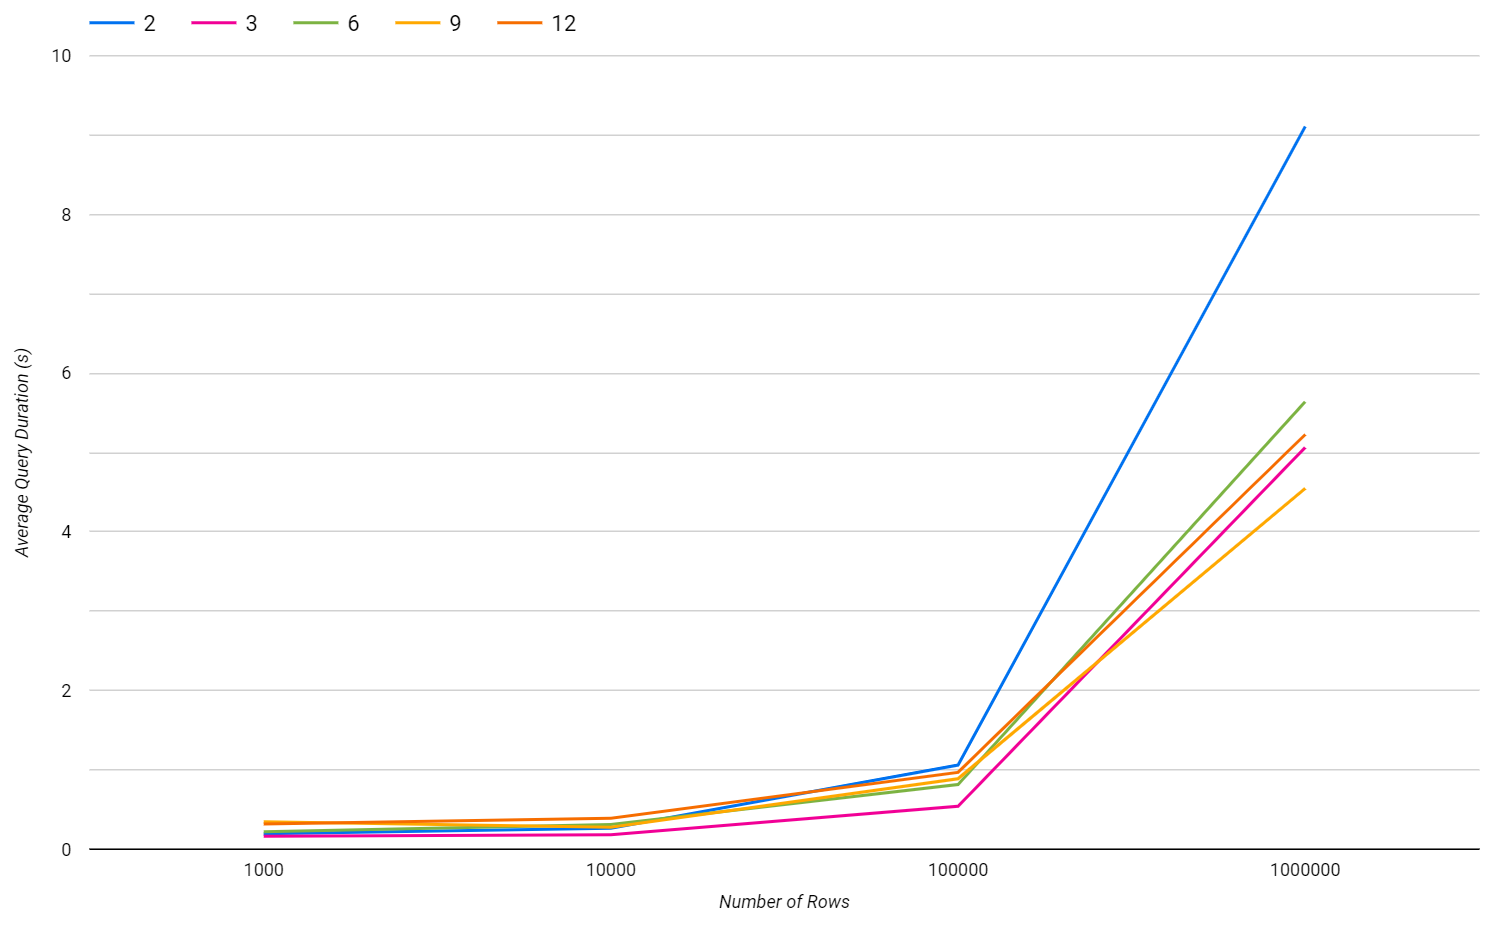
\includegraphics[width=0.8\linewidth]{chapters/diagrams/testing/filter-simple-parallelisation-test}
	\caption{Parallelisation - Filter Query Results}
	\label{fig:filter-simple-parallelisation-test}
\end{figure}

\begin{figure}[ht]
	\centering
	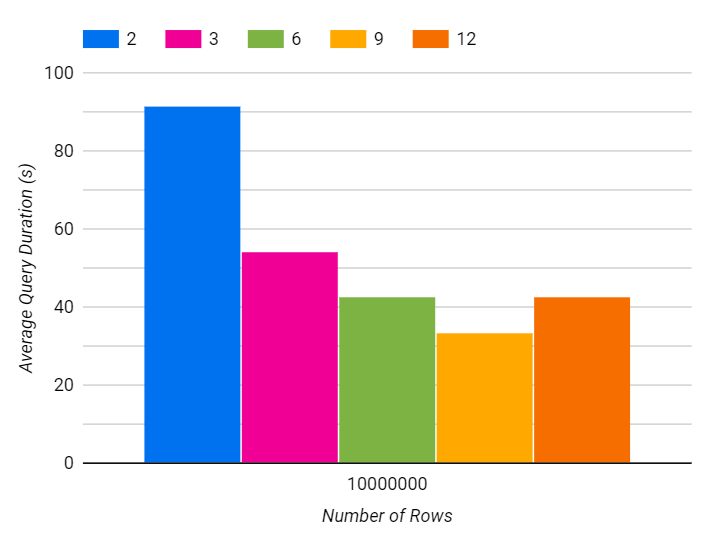
\includegraphics[width=0.4\linewidth]{chapters/diagrams/testing/filter-simple-parallelisation-10m}
	\caption{Parallelisation - Filter Query Results, 10 Million Rows}
	\label{fig:filter-simple-parallelisation-10m}
\end{figure}

\subsection{Group By Query}
The results of this test are shown in Figure \ref{fig:group-by-simple-parallelisation-test}. These results again suggest that there is a balancing point for the level of parallelisation. The 3 node cluster is consistently faster than all other cluster layouts. The 6, 9 and 12 cluster layouts are likely to be slower because increasing the level of parallelisation will result in higher amounts of cross-communication, and network transfer is one of the slowest areas, as identified in the SQL test.

Interestingly, the 2 node cluster is second fastest until 1 million rows, when its performance significantly reduces. This is likely to be because the increased memory demands on each node caused by having fewer worker nodes resulted in some data being spilled to disk, which results in reduced query performance.

\begin{figure}[ht]
	\centering
	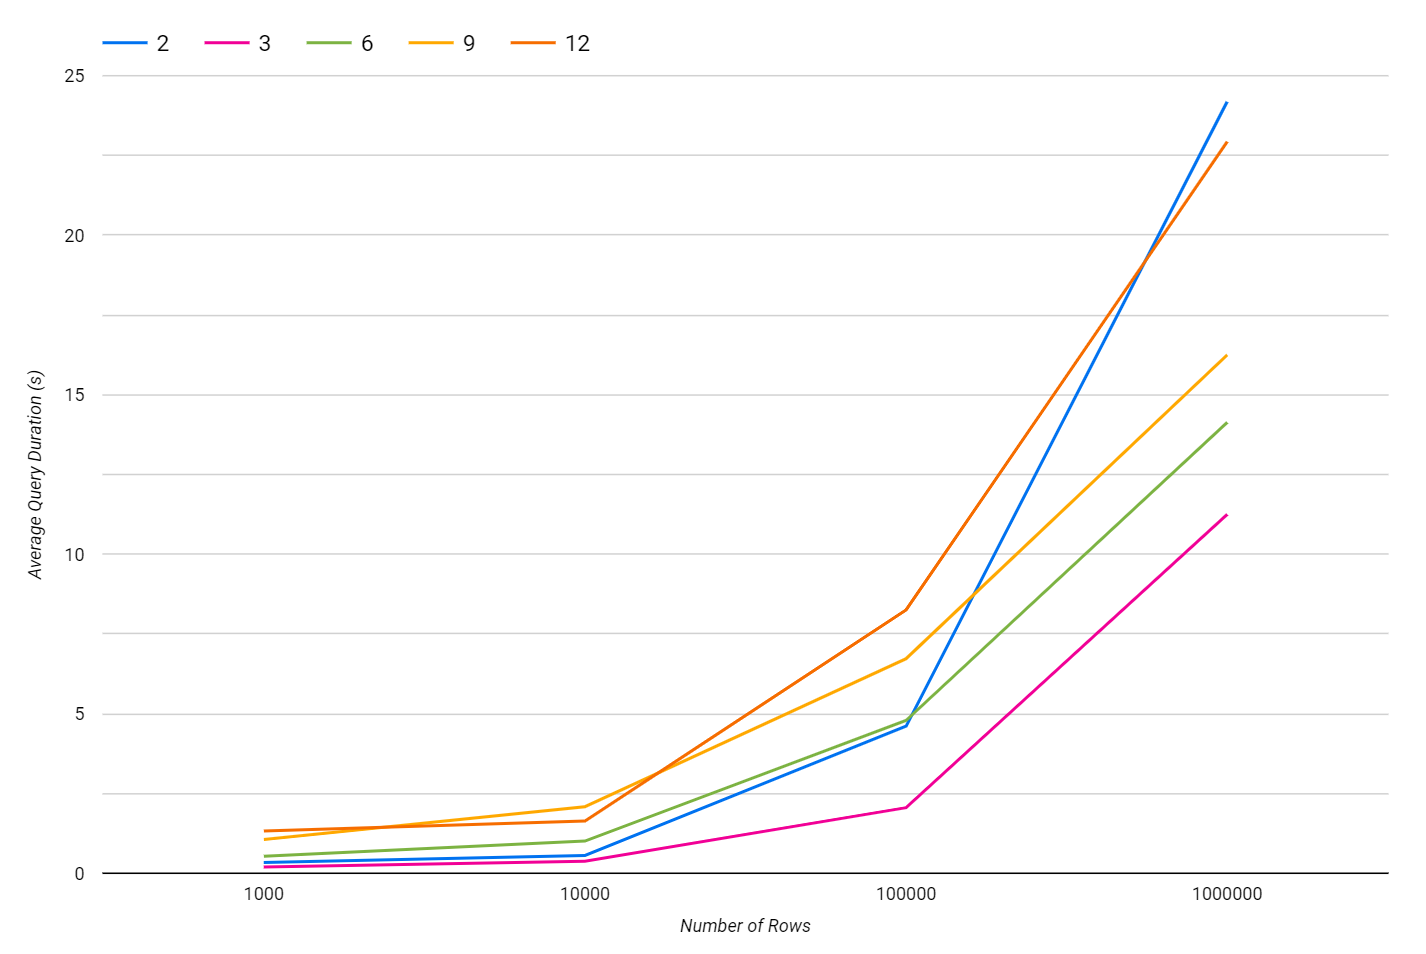
\includegraphics[width=0.8\linewidth]{chapters/diagrams/testing/group-by-simple-parallelisation-test}
	\caption{Parallelisation - Group By Query Results}
	\label{fig:group-by-simple-parallelisation-test}
\end{figure}

\subsection{Analysis}
Overall, the outcomes of this test show that there is no clear solution to the number of nodes in the cluster. As a general rule, matching the number of workers to the number of Cassandra nodes in the cluster will result in good performance, but the Filter test also shows that increasing the level of parallelisation can result in better performance for the same resources at larger query sizes. Solutions to this problem depend entirely on the queries being run, and the data volumes the queries are applied to. There is an opportunity for further research designing a system that can analyse the queries being executed, and adjust the cluster layout to match the requirements of those queries.

\section{Autoscaling}
This section will compare computation speed of the Cluster Processor when the overall performance is reduced. The motivation for the test is the autoscaling feature present in many managed Kubernetes services, including Azure Kubernetes Service, which continually analyses the load of the Kubernetes cluster, and increases or decreases the number of physical nodes based on current demand \cite{aksautoscaling}. By doing this, applications with fluctating levels of demand are able to save costs by reducing the number of machines they pay for in periods of low demand.

While the Cluster Processor is not currently implemented in a way that supports autoscaling, this test is performed to identify how effective autoscaling would be on this solution. In these tests the simple versions of the Select, Filter and Group By queries were executed, with a different range of rows depending on the test. Figure \ref{fig:autoscale-test-workers} shows the cluster layouts for each test case; the number of workers, and the resources available to each worker. Each cluster layout has one less worker, and 33\% less resources available.

Throughout all of these tests, the number of Cassandra nodes in the cluster remained consistent: 3 nodes, one placed on each Kubernetes node.

\begin{figure}[ht]
	\centering
	\begin{tabular}{| c | c | c | c | c |}
		\hline
		\textbf{Workers} & \textbf{vCores} & \textbf{Worker Memory} & \textbf{Total vCores} & \textbf{Total Memory} \\ \hline
		3 & 2 & 6GB & 6 & 18GB \\ \hline
		2 & 2 & 6GB & 4 & 12GB \\ \hline
		1 & 2 & 6GB & 2 & 6GB \\ \hline
	\end{tabular}
	\caption{Autoscaling - Number of Workers and Resources}
	\label{fig:autoscale-test-workers}
\end{figure}

\subsection{Select Query}
The results of this test are shown in Figure \ref{fig:select-simple-autoscale-test}. As expected, the query performance decreases as the number of workers decreases. However, at 1000 rows the difference between 3 workers and 1 worker is around 0.3s, and at 10000 rows it is 0.9s

\begin{figure}[ht]
	\centering
	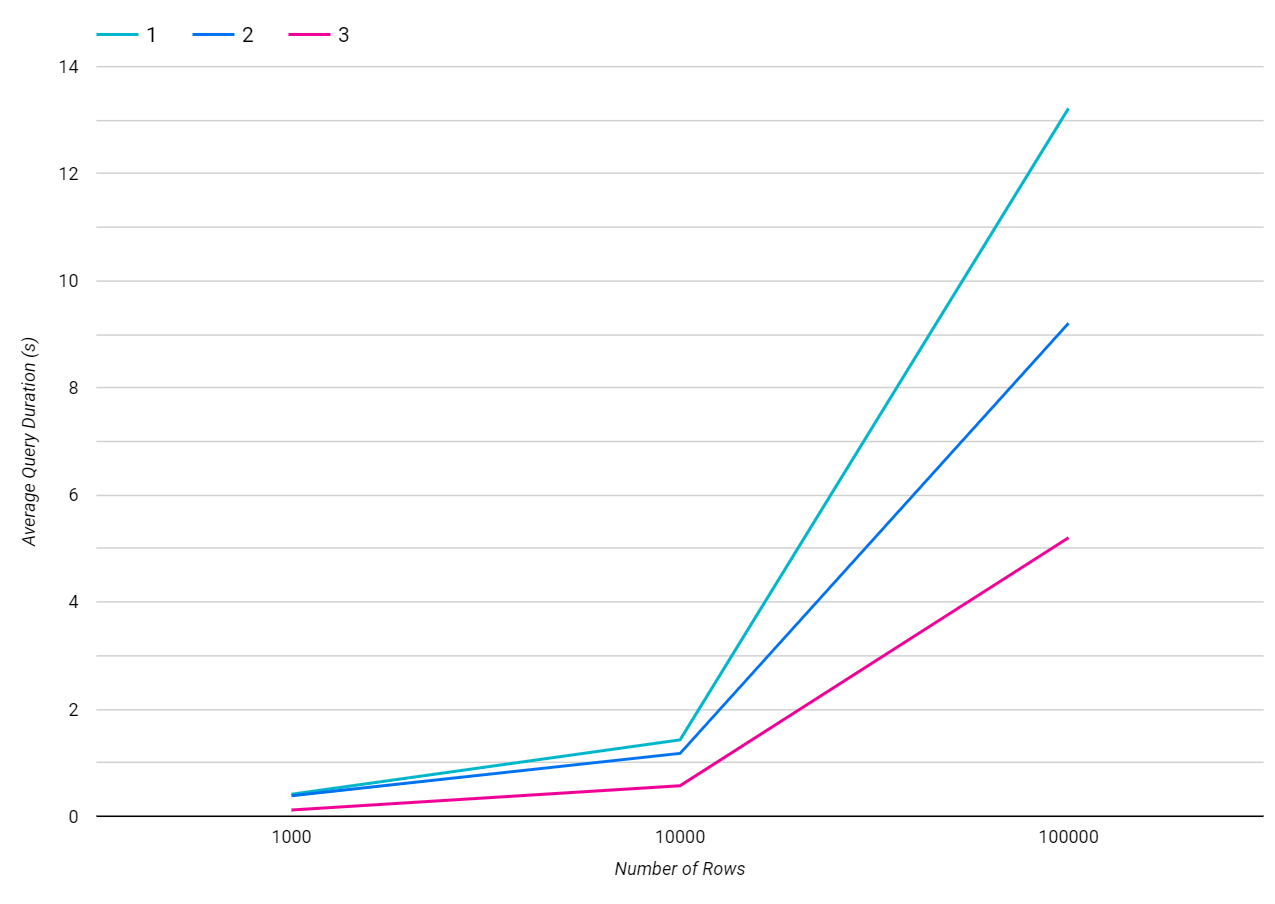
\includegraphics[width=0.8\linewidth]{chapters/diagrams/testing/select-simple-autoscale-test}
	\caption{Autoscaling - Select Query Results}
	\label{fig:select-simple-autoscale-test}
\end{figure}

\subsection{Filter Query}
The results of this test are shown in Figure \ref{fig:filter-simple-autoscale-test}. As before, the query performance decreases as the number of workers decreases. However, at small data volumes the difference between 1 and 3 workers is even smaller than in the Select test. The difference between 1 and 3 workers is 0.08s at 1000 rows, 0.2s at 10000 rows, and 1.1s at 100,000 rows.

\begin{figure}[ht]
	\centering
	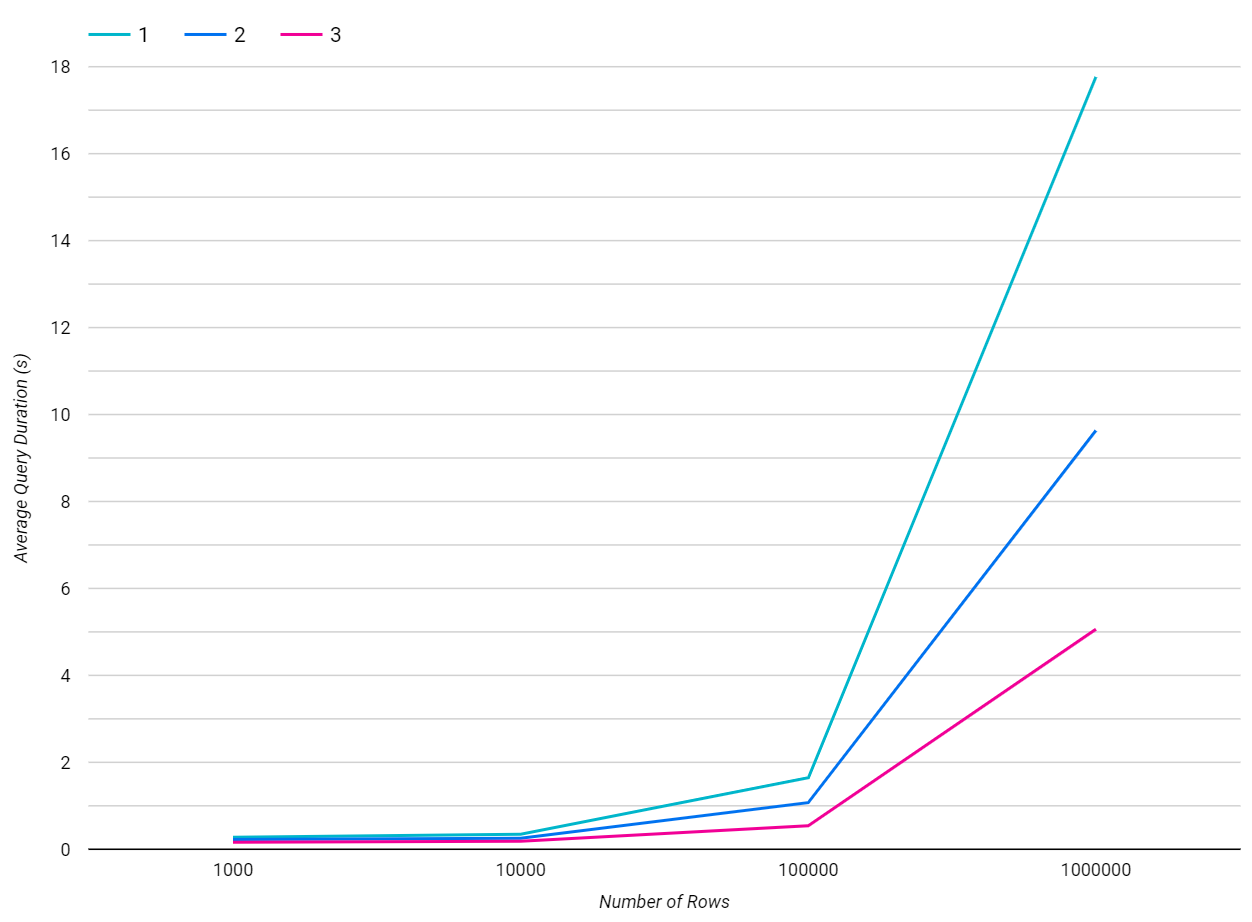
\includegraphics[width=0.8\linewidth]{chapters/diagrams/testing/filter-simple-autoscale-test}
	\caption{Autoscaling - Filter Query Results}
	\label{fig:filter-simple-autoscale-test}
\end{figure}

\subsection{Group By Query}
The results of this test are shown in Figure \ref{fig:group-by-simple-autoscale-test}. At 1000 and 10000 rows, there is effectively no difference between the three cluster layouts, and at 100000 rows the 1 node cluster is the fastest by 0.5s on average. Once the data volume increases to 1 million rows, the 3 node cluster is significantly faster than the other two layouts. However, these results suggest that, at very small data volumes, it is faster to perform all of the computation on a single node. This is because it prevents the need for the workers to cross-communicate, and if all data can be kept in memory, the computation will be performed significantly faster.

\begin{figure}[ht]
	\centering
	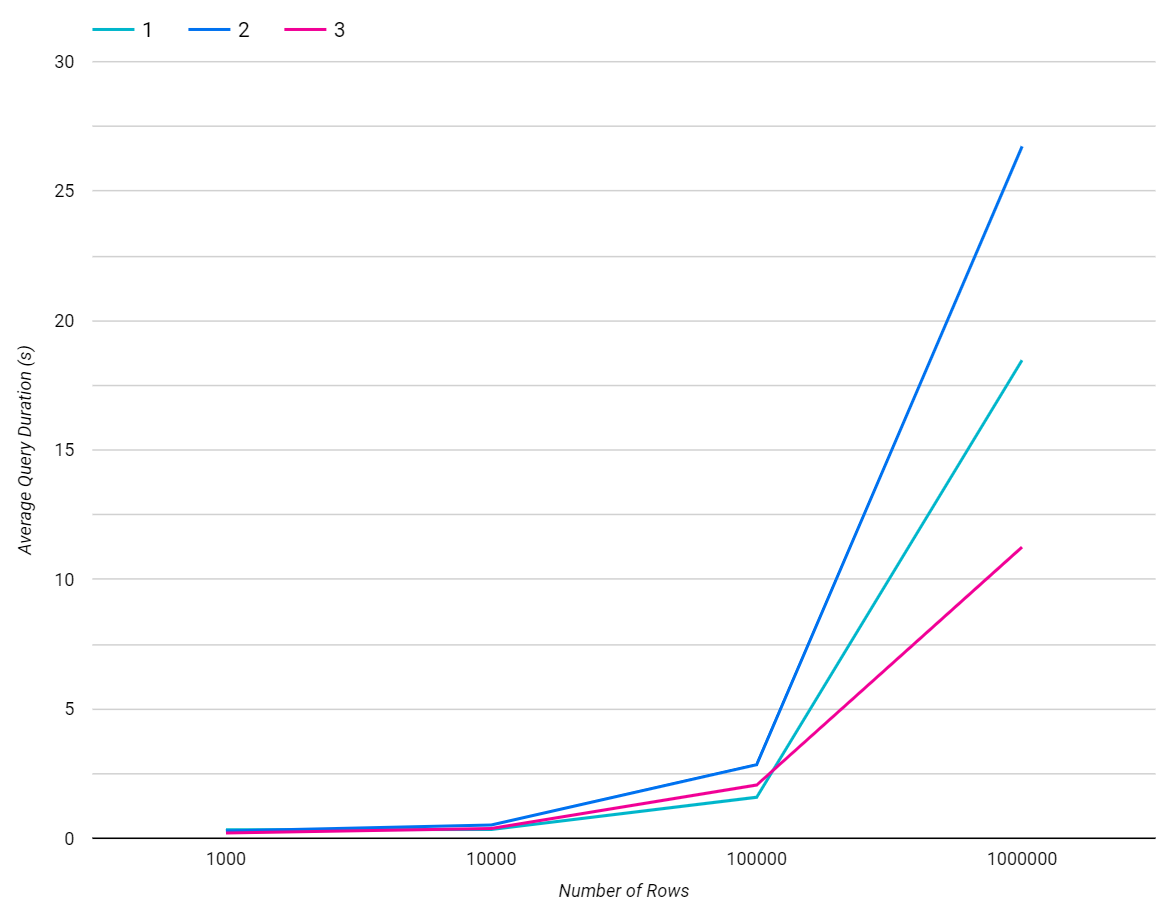
\includegraphics[width=0.8\linewidth]{chapters/diagrams/testing/group-by-simple-autoscale-test}
	\caption{Autoscaling - Group By Query Results}
	\label{fig:group-by-simple-autoscale-test}
\end{figure}

\subsection{Analysis}
The outcomes of this test show that it is effective to reduce the cluster size if the data volumes are small. The time difference between the smallest and largest cluster is typically less than a second when operating on less than 1 million rows. This is insignificant for most use cases, and if a time-critical system was reliant on querying this small amount of data, a more typical solution like SQL would be better suited to solve the problem regardless.

	
	\chapter{Evaluation}\label{cha:evaluation}
This section will discuss a high level evaluation of the solution, and the project as a whole.

\section{Limitations}
The solution has limitations which could not be fixed due to time constraints, but further investigation into optimisations or alternative solutions may be able to improve or fix them. These are listed below.

As discussed in Chapter \ref{cha:testing}, the Group By operation, and the method of transferring data around the network could both be further optimised.

%Firstly, transferring data over the network is common in the distributed system model. In particular, this occurs when returning final result data to the orchestrator and frontend, as well as when cross-communicating between workers. However, the performance testing identified that this is one of the weakest areas of the implementation. Therefore, optimising this process would be a focus in future development.

%The current implementations of Group Bys are computationally correct, but not as efficient as they could be. Currently, when partial data for a partition is communicated between workers, all rows from the source data are sent over the network. As the data transfer solution also has relatively poor performance, sending unnecessary data between workers exacerbates the issue. It should be possible to partially compute each group by during the hash calculation phase, then only send the partially computed result, which is then compiled by the worker that is responsible for the final partition. 

Result data uses an extremely large amount of space when resident in memory. For example, a 100MB source data file can use up to 800MB of memory once stored. This is because of the container class described in Section \ref{sec:type-system}. However, this class is a core component of the DSL, as it ensures the type information is accessible at runtime.

The system's security is limited, which prevents its use in a production environment. The orchestrator has no authentication, and Cassandra only has basic username and password authentication.

Finally, as discovered in Chapter \ref{cha:testing}, the result collation algorithm cannot return large amounts of results, typically more than 1 million rows. All workers send results to the orchestrator, which forwards them to the frontend. However, as there are more workers than the single orchestrator, data enters the orchestrator faster than it leaves, meaning that with a large enough dataset, the orchestrator will run out of memory and crash.

\section{Further Work}
The nature of this project means that there is a large scope for future work and improvements. As discussed in Section \ref{sec:parallelisation-test}, different cluster layouts are more optimised for different kinds of queries. 
%Queries with less computation, or that run on smaller amounts of data are better applied to smaller clusters, while increasing the level of parallelisation is better when the query is larger or more complex.
A module that runs at the Kubernetes level, monitoring the utilisation of the cluster and the types of queries being executed may be able to improve computation times by adjusting the cluster layout.

The data store is currently used to assist computations by temporarily storing partial result data. However, the design would allow it to store results between queries, improving the computation time of repeated queries to the same dataset. Join operations are also not currently implemented, but would benefit from this improvement to the data store. 

The current error handling is designed to forward any errors to the frontend. In some situations, like if the Cassandra database is unresponsive, this is acceptable. For other errors, like if one worker is unresponsive, this can be handled by delegating the failed worker's partitions to others, without alerting the user at all.

Finally, Cassandra is currently only used for storage and partitioning. However, it is also a query engine, meaning some computations could be performed on Cassandra directly, improving query times by reducing the amount of data transferred. In particular, Filters on the source dataset, and Group Bys on the primary key are perfect candidates for this optimisation.

% Personal analysis?? not present in other projects
% - Software Engineering Processes - CI/CD
% - Architecture
% - Approach (MVP first)

\section{Conclusion}
The objective as stated in Chapter \ref{cha:intro} was to design a query processing engine for a distributed cluster of nodes. The types of queries possible in the system are numerous, and the data model allows easy implementation of new query types. While performance testing results showed that the solution requires further optimisation to truly compete with existing frameworks, they also showed that there is promise in the scalability of the solution. Furthermore, testing revealed interesting findings regarding the number of workers in the cluster, and raised the possibility of a stand-alone module for performing node management. 

A secondary goal was to design the frontend to be easy-to-use, with SQL-like syntax. The DSL meets this goal, and is one of the defining features of the tool, with \textit{FieldExpressions} and \textit{FieldComparisons} allowing complex data manipulations to be defined with relative ease. The implementation of Functions permits easy extensions within the type system's bounds. The frontend operates seamlessly for the user, hiding the background operation of the framework entirely. Furthermore, the pandas integration means that users can immediately start manipulating result data using tools already familiar to them.
	
	\listoftodos
	
	{
		\backmatter
		\printbibliography
	}
	
	\appendix
	
	\chapter{Testing Figures}\label{cha:testing-figs}

Included in this appendix are figures with the queries used for performance testing.

\begin{figure}[h]
	\centering
	\begin{SQL}
SELECT * FROM data.origination_1000
	\end{SQL}
	\caption{SQL - Select Simple}
	\label{fig:sql-select-simple}
\end{figure}
	
\begin{figure}[h]
	\begin{python}
manager = ClusterManager("orchestrator-service")
manager.cassandra_table("data", "origination_1000").evaluate()
	\end{python}
	\caption{Cluster Processor - Select Simple}
	\label{fig:cluster-select-simple}
\end{figure}

\begin{figure}[h]
	\centering
	\begin{SQL}
SELECT 
Loan_ID + 1 as Loan_ID_Inc, 
interest_rate + 1 as Interest_rate_Inc, 
power(duration, 2) as Duration_Pow, 
substring(cast(origination_date as nvarchar(300)), 0, 11) as origination_date_str 
FROM data.origination_1000
	\end{SQL}
	\caption{SQL - Select Complex}
	\label{fig:sql-select-complex}
\end{figure}

\begin{figure}[h]
	\begin{python}
manager = ClusterManager("orchestrator-service")
manager.cassandra_table("data", "origination_1000").select(
(F("loan_id") + 1).as_name("loan_id_inc"), 
(F("interest_rate") + 1).as_name("interest_rate_inc"),
Function.Pow(Function.ToDouble(F("duration")), 2.0).as_name("duration_pow"),
Function.Substring(Function.ToString(F("origination_date")), 0, 10).as_name("orignation_date_str")
).evaluate()
	\end{python}
	\caption{Cluster Processor - Select Complex}
	\label{fig:cluster-select-complex}
\end{figure}

\begin{figure}[h]
	\centering
	\begin{SQL}
SELECT *
FROM data.origination_1000
WHERE duration = 30
	\end{SQL}
	\caption{SQL - Filter Simple}
	\label{fig:sql-filter-simple}
\end{figure}

\begin{figure}[h]	
	\begin{python}
manager = ClusterManager("orchestrator-service")
manager.cassandra_table("data", "origination_1000")
.filter(F("duration") == 30)
.evaluate()
	\end{python}
	\caption{Cluster Processor - Filter Simple}
	\label{fig:cluster-filter-simple}
\end{figure}

\begin{figure}[h]
	\centering
	\begin{SQL}
SELECT *
FROM data.origination_1000
WHERE 
(duration = 30 AND amount > 500000)
OR loan_id = 1
	\end{SQL}
	\caption{SQL - Filter Complex}
	\label{fig:sql-filter-complex}
\end{figure}
	
\begin{figure}[h]
	\begin{python}
manager = ClusterManager("orchestrator-service")
manager.cassandra_table("data", "origination_1000")
.filter(
((F("duration") == 30) & (F("amount") > 500000.0))
| (F("loan_ID") == 1)
).evaluate()
	\end{python}
	\caption{Cluster Processor - Filter Complex}
	\label{fig:cluster-filter-complex}
\end{figure}

\begin{figure}[h]
	\centering
	\begin{SQL}
		SELECT duration
		FROM data.origination_1000
		GROUP BY duration
	\end{SQL}
	\caption{SQL - Group By Simple}
	\label{fig:sql-group-by-simple}
\end{figure}

\begin{figure}[h]
	\begin{python}
manager = ClusterManager("orchestrator-service")
manager.cassandra_table("data", "origination_1000")
.group_by([F("duration")])
.evaluate()
	\end{python}
	\caption{Cluster Processor - Group By Simple}
	\label{fig:cluster-group-by-simple}
\end{figure}

\begin{figure}[h]
	\centering
	\begin{SQL}
SELECT 
duration, 
MAX(origination_date) as Max_origination_date, 
AVG(interest_rate) as Avg_interest_rate, 
Min(amount) as Min_amount 
FROM data.origination_1000 
GROUP BY duration
	\end{SQL}
	\caption{SQL - Group By Complex}
	\label{fig:sql-group-by-complex}
\end{figure}

\begin{figure}[h]
	\begin{python}
manager = ClusterManager("orchestrator-service")
manager.cassandra_table("data", "origination_1000")
.group_by(
[F("duration")],
[	Max(F("origination_date")), 
Avg(F("interest_rate")), 
Min(F("amount"))
]
).evaluate()
	\end{python}
	\caption{Cluster Processor - Group By Complex}
	\label{fig:cluster-group-by-complex}
\end{figure}
	
	
\end{document}